%%%%%%%%%%%%%%%%%%%%%%%%%%%%%%%%%%%%%%%%%%%%%%%%%%%%%%%%%%%%%%%%%%%%%%%%%%%%%%%%
%%  Permanent Set Model
%%%%%%%%%%%%%%%%%%%%%%%%%%%%%%%%%%%%%%%%%%%%%%%%%%%%%%%%%%%%%%%%%%%%%%%%%%%%%%%%


\section{Permanent set model}

%%%%%%%%%%%%%%%%%%%%%%%%%%%%%%%%%%%%%%%%%%%%%%%%%%%%%%%%%%%%%%%%%%%%%%%%%%%%%%%%
%%%%    Kinematics

\subsection{Kinematics}

	For the bulk tissue level mechanical response, consisting of the EXL matrix, the collagen fibers, and fiber ensemble interactions, we first consider the EXL matrix alone. Permanent set occurs in the EXL matrix, and is the main driver for the evolving mechanical response and structural changes in the tissue. As such the permanent set model is our starting point (section \ref{sec:modelapproach}), which then can be used to convect collagen fiber architecture and predict the remaining collagen fibers and fiber ensemble interactions components of the mechanical response. To model the EXL matrix under permanent set, many reference states need to be considered. Due to scission-healing, the reference configuration of the EXL matrix is the configuration at its time of formation. For this we first introduce the following definition for the for the evolution of the configurations involved (Fig. \ref{fig:stateevolution}):

\begin{enumerate}

\item The original unloaded configuration $\Omega_0$ 

\item The evolving loaded configuration is $\Omega(s)$, where $s$ is the current time. 

\item We also make the distinction between $\hat{s}$, the intermediate time for which the EXL matrix is formed, and $s$. As the reference configuration of the EXL matrix evolves, there needs to be a distinction between the configuration for which the EXL matrix formed by the scission-healing reaction at time $\hat{s}$, referenced to $\Omega(\hat{s})$, and the current loaded configuration $\Omega(s)$. In this way, $\hat{s}$ is also suitable as an variable of integration.

\item The strain history, $\mathbf{A}(s)$, which is a deformation gradient tensor as a function of time $s$, that maps between the original configuration $\Omega_0$ to the loaded configuration $\Omega(s)$ at which the EXL matrix is formed

\item We define $\tilde{\mathbf{B}}(s) = \mathbf{A}\mathbf{A}^\mathsf{T}$ to be left Cauchy Green tensor of the strain history $\mathbf{A}(s)$, which should not be confused with the left Cauchy Green tensor of the deformation applied to the tissue

\item We define the deformation gradient tensor from the intermediate loaded state $\Omega(\hat{s})$ to the current loaded state $\Omega(s)$ to be $\mathbf{\bar{F}}(\hat{s})$, where the following relation is assumed (Fig. \ref{fig:stateevolution})
\begin{equation} \label{eq:strainhistory}
\begin{split}
&\mathbf{F} = \mathbf{\bar{F}}(\hat{s})\mathbf{A}(\hat{s}), \\
&\mathbf{\bar{F}}(\hat{s}) = \mathbf{F} \cdot \mathbf{A}(\hat{s})^{-1}.
\end{split}
\end{equation}

\item The evolving unloaded reference configuration after permanent set is $\Omega_\mathrm{PS}(s)$ with $\mathbf{F}_\mathrm{PS}(s)$ mapping from the original configuration $\Omega_0$ to $\Omega_\mathrm{PS}(s)$

\end{enumerate}

\begin{figure}[hbt]
\centering
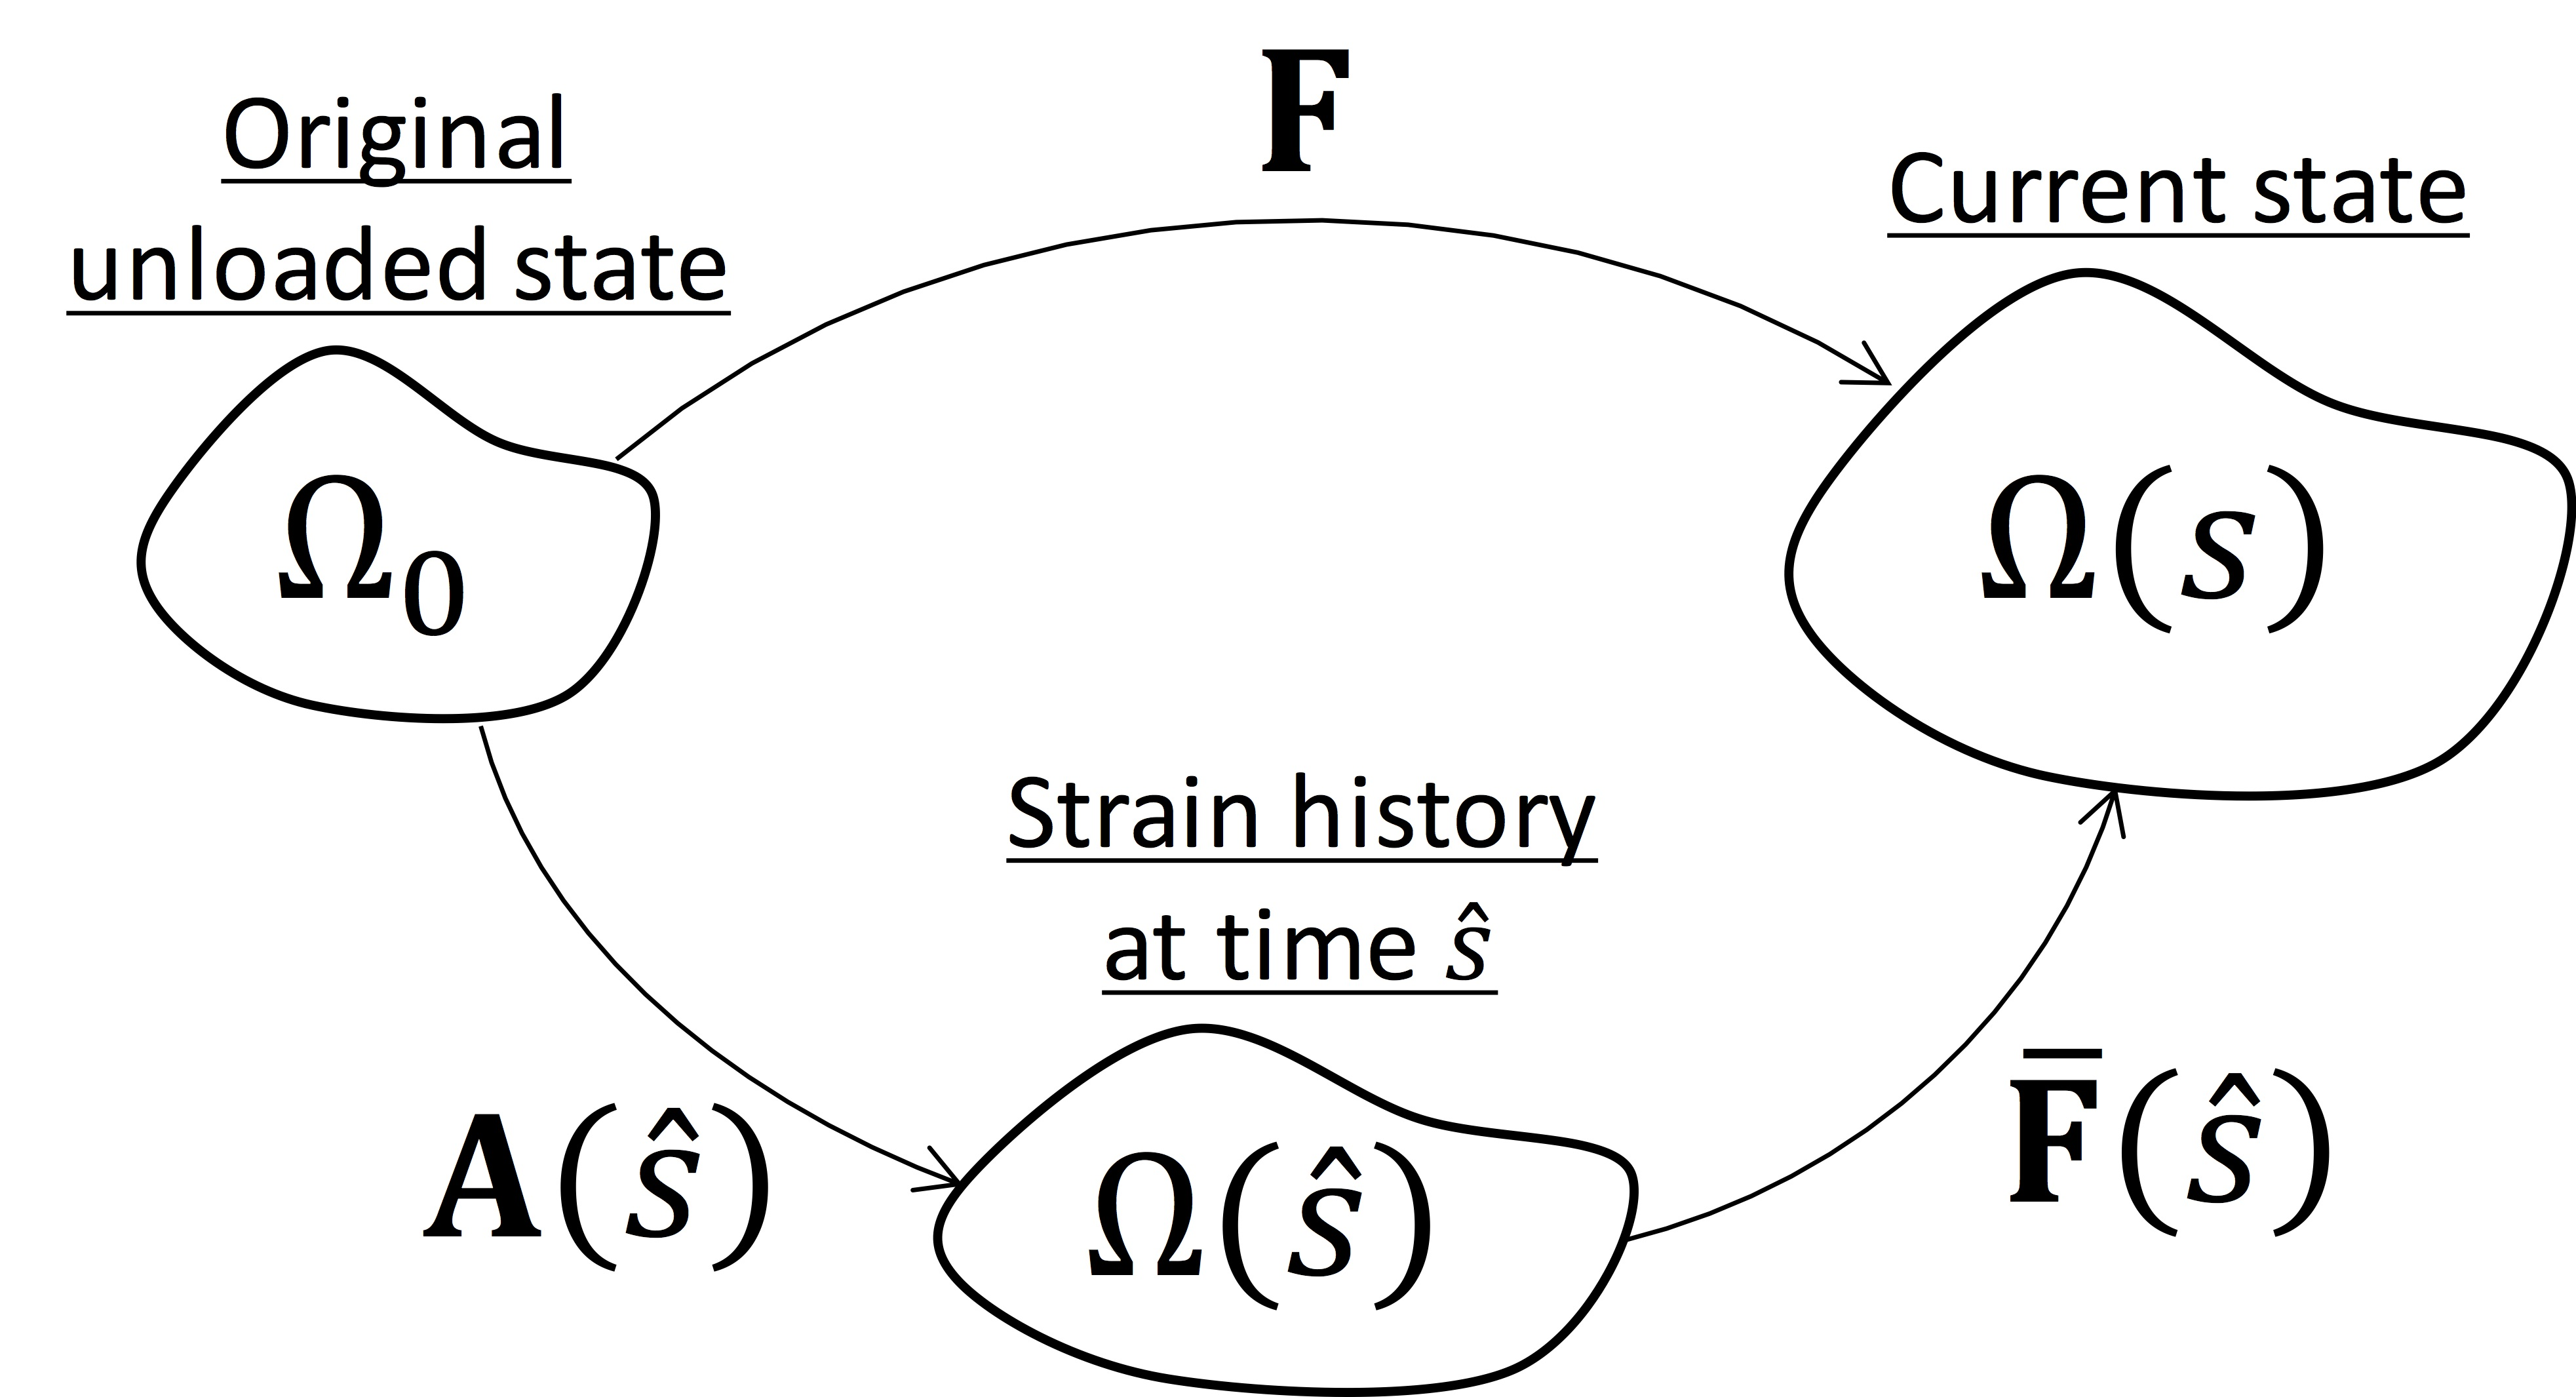
\includegraphics[width=3.5in]{Images/chapter4/figure7}
\caption{The relation between the reference configurations during cyclic loading.}
\label{fig:stateevolution}
\end{figure}

    We also note the following important considerations:
\begin{itemize}
\item The original reference configuration $\Omega_0$ is important as it is the configuration for which the mechanical response of the original material as well as the collagen fiber architecture is referenced. Similarly, we track the loaded configuration ($\Omega(s)$) using $\mathbf{A}(s)$ and the unloaded configuration ($\Omega_\mathrm{PS}(s)$) using $\mathbf{F}_\mathrm{PS}$ from $\Omega_0$. 

\item We also note that under cyclic loading, the exogenously crosslinked tissue is not held at the constant loaded configuration, it is put through a range of deformation each cycle. Because permanent set happens at a time scale much longer than a single cycle, we define the loaded configuration $\Omega(s)$ as the root mean squared configuration, which is the time averaged deformation for a single loading cycle. 

\item We note that the tissue is never fully unloaded during cyclic loading. Thus, to simulate cyclic loading, the stresses are still referenced to the origin configuration $\Omega_0$. The unloaded geometry is determined \textit{a posteriori} from $\Omega_\mathrm{PS}(s)$ for when cyclic loading is stopped for mechanical testing. 
\end{itemize}



    Thus the right Cauchy Green tensor when referenced to the strain history $\Omega(\hat{s})$ is given by $\mathbf{\bar{C}}(\hat{s}) = \mathbf{\bar{F}}(\hat{s})^\mathsf{T} \mathbf{\bar{F}}(\hat{s})$. This also has the following relation to the applied deformation $\mathbf{F}$,
\begin{equation} \label{eq:rightcauchy}
\begin{split}
\mathbf{\bar{C}}(\hat{s}) &= \left( \mathbf{F}\cdot\mathbf{A}(\hat{s})^{-1} \right)^\mathsf{T} \left(\mathbf{F} \cdot \mathbf{A}(\hat{s})^{-1} \right)\\
	&= \mathbf{A}(\hat{s})^{-\mathsf{T}} \left( \mathbf{F}^\mathsf{T} \mathbf{F} \right) \mathbf{A}(\hat{s})^{-1} \\
	&= \mathbf{A}(\hat{s})^{-\mathsf{T}} \cdot \mathbf{C} \cdot \mathbf{A}(\hat{s})^{-1}.
\end{split}
\end{equation}
    Our material model for the EXL matrix is an isotropic model of $\Psi_m = \Psi_m(I_1)$, where $I_1$ is the first invariant of $\mathbf{C}$. For this, we can define the first invariant $\bar{I}_1(\hat{s})$ for the right Cauchy Green tensor $\bar{\mathbf{C}}(\hat{s})$ as 
\begin{equation}\label{eq:pseudo1stinv}
\bar{I}_1(\hat{s}) = \operatorname{Trace}(\mathbf{\bar{C}}(\hat{s})) = \operatorname{Trace}\left(\mathbf{A}^{-\mathsf{T}}(\hat{s}) \cdot \mathbf{C} \cdot \mathbf{A}^{-1}(\hat{s})\right).
\end{equation}
    With this, the stress of the EXL matrix is given by 

\begin{equation}
\mathbf{\bar{S}}_m = 2 \frac{\partial \bar{\Psi}}{\partial \mathbf{C}} - p\mathbf{I} = 2 \frac{\partial \bar{\Psi}}{\partial \bar{I}_1(\hat{s})} \frac{\partial \bar{I}_1(\hat{s})}{\partial \mathbf{C}} - p\mathbf{I},
\end{equation}
    where $p$ is the Lagrange multiplier enforcing incompressibility. The partial derivative of $\bar{I}_1(\hat{s})$ is
\begin{equation}
\frac{\partial\bar{I}_1}{\partial\mathbf{C}} = \frac{\partial\bar{I}_1}{\partial\bar{\mathbf{C}}(\hat{s})} \frac{\partial\bar{\mathbf{C}}(\hat{s})}{\partial \mathbf{C}}= \frac{\partial\mathbf{A}(\hat{s})^{-\mathsf{T}} \cdot \mathbf{C} \cdot \mathbf{A}(\hat{s})^{-1}}{\partial \mathbf{C}} = \mathbf{A}(\hat{s})^{-\mathsf{T}} \mathbf{A}(\hat{s})^{-1} = \mathbf{\tilde{B}}(\mathbf{A}(\hat{s}))^{-1},
\end{equation}
    which is the inverse of the left Cauchy Green tensor of the strain history $\mathbf{A(s)}$.


%%%%%%%%%%%%%%%%%%%%%%%%%%%%%%%%%%%%%%%%%%%%%%%%%%%%%%%%%%%%
%%%%%%      Constitutive Model for crosslinking

\subsubsection{Kinematics for updating the reference configuration}

    As the unloaded configuration changes due to permanent set, we need to be able to express the stresses with the new reference configuration. Since all configurations are referenced to $\Omega_0$, the deformation from the new reference configuration $\Omega_\mathrm{PS}$ to the current loaded state $\Omega(s)$ is given by (Fig. \ref{fig:PSevolution})
\begin{equation}
\mathbf{F} = \mathbf{\bar{F}}(\hat{s}) \cdot \mathbf{A}(\hat{s}) \cdot \mathbf{F}_\mathrm{PS}^{-1}.
\end{equation}
    Following the same derivation as equations \ref{eq:strainhistory}--\ref{eq:pseudo1stinv}, we have
\begin{equation} \label{eq:newhistory}
\begin{split}
\mathbf{\bar{F}}(\hat{s}) &= \mathbf{F} \cdot \mathbf{F}_\mathrm{PS} \cdot \mathbf{A}(\hat{s})^{-1},\\
\mathbf{\bar{C}}(\mathbf{F}_\mathrm{PS}, \mathbf{A}(\hat{s})) &= \mathbf{A}(\hat{s})^{-\mathsf{T}} \cdot \mathbf{F}_\mathrm{PS}^\mathsf{T} \cdot \mathbf{C} \cdot \mathbf{F}_\mathrm{PS} \cdot \mathbf{A}(\hat{s})^{-1}, \\
\bar{I}_1\left(\mathbf{F}_\mathrm{PS}, \mathbf{A}(s)\right) &= \operatorname{Trace}\left(\mathbf{A}(\hat{s})^{-\mathsf{T}} \cdot \mathbf{F}_\mathrm{PS}^\mathsf{T} \cdot \mathbf{C} \cdot \mathbf{F}_\mathrm{PS} \cdot \mathbf{A}(\hat{s})^{-1}\right). 
\end{split}
\end{equation}
    and the new inverse of the left Cauchy Green tensor of the strain history is given by
\begin{equation}
\begin{split}
\mathbf{\tilde{B}}(\mathbf{F}_\mathrm{PS}, \mathbf{A}(\hat{s}))^{-1} &= \frac{\partial \mathbf{\bar{C}}(\mathbf{F}_\mathrm{PS}, \mathbf{A}(\hat{s}))}{\partial \mathbf{C}} = \frac{\mathbf{A}(\hat{s})^{-\mathsf{T}} \cdot \mathbf{F}_\mathrm{PS}^\mathsf{T} \cdot \mathbf{C} \cdot \mathbf{F}_\mathrm{PS} \cdot \mathbf{A}(\hat{s})^{-1}}{\partial \mathbf{C}} \\
 &= \mathbf{A}(\hat{s})^{-\mathsf{T}} \cdot \mathbf{F}_\mathrm{PS}^\mathsf{T} \cdot \mathbf{F}_\mathrm{PS} \cdot \mathbf{A}(\hat{s})^{-1}. 
\end{split}
\end{equation}

\begin{figure}[hbt]
\centering
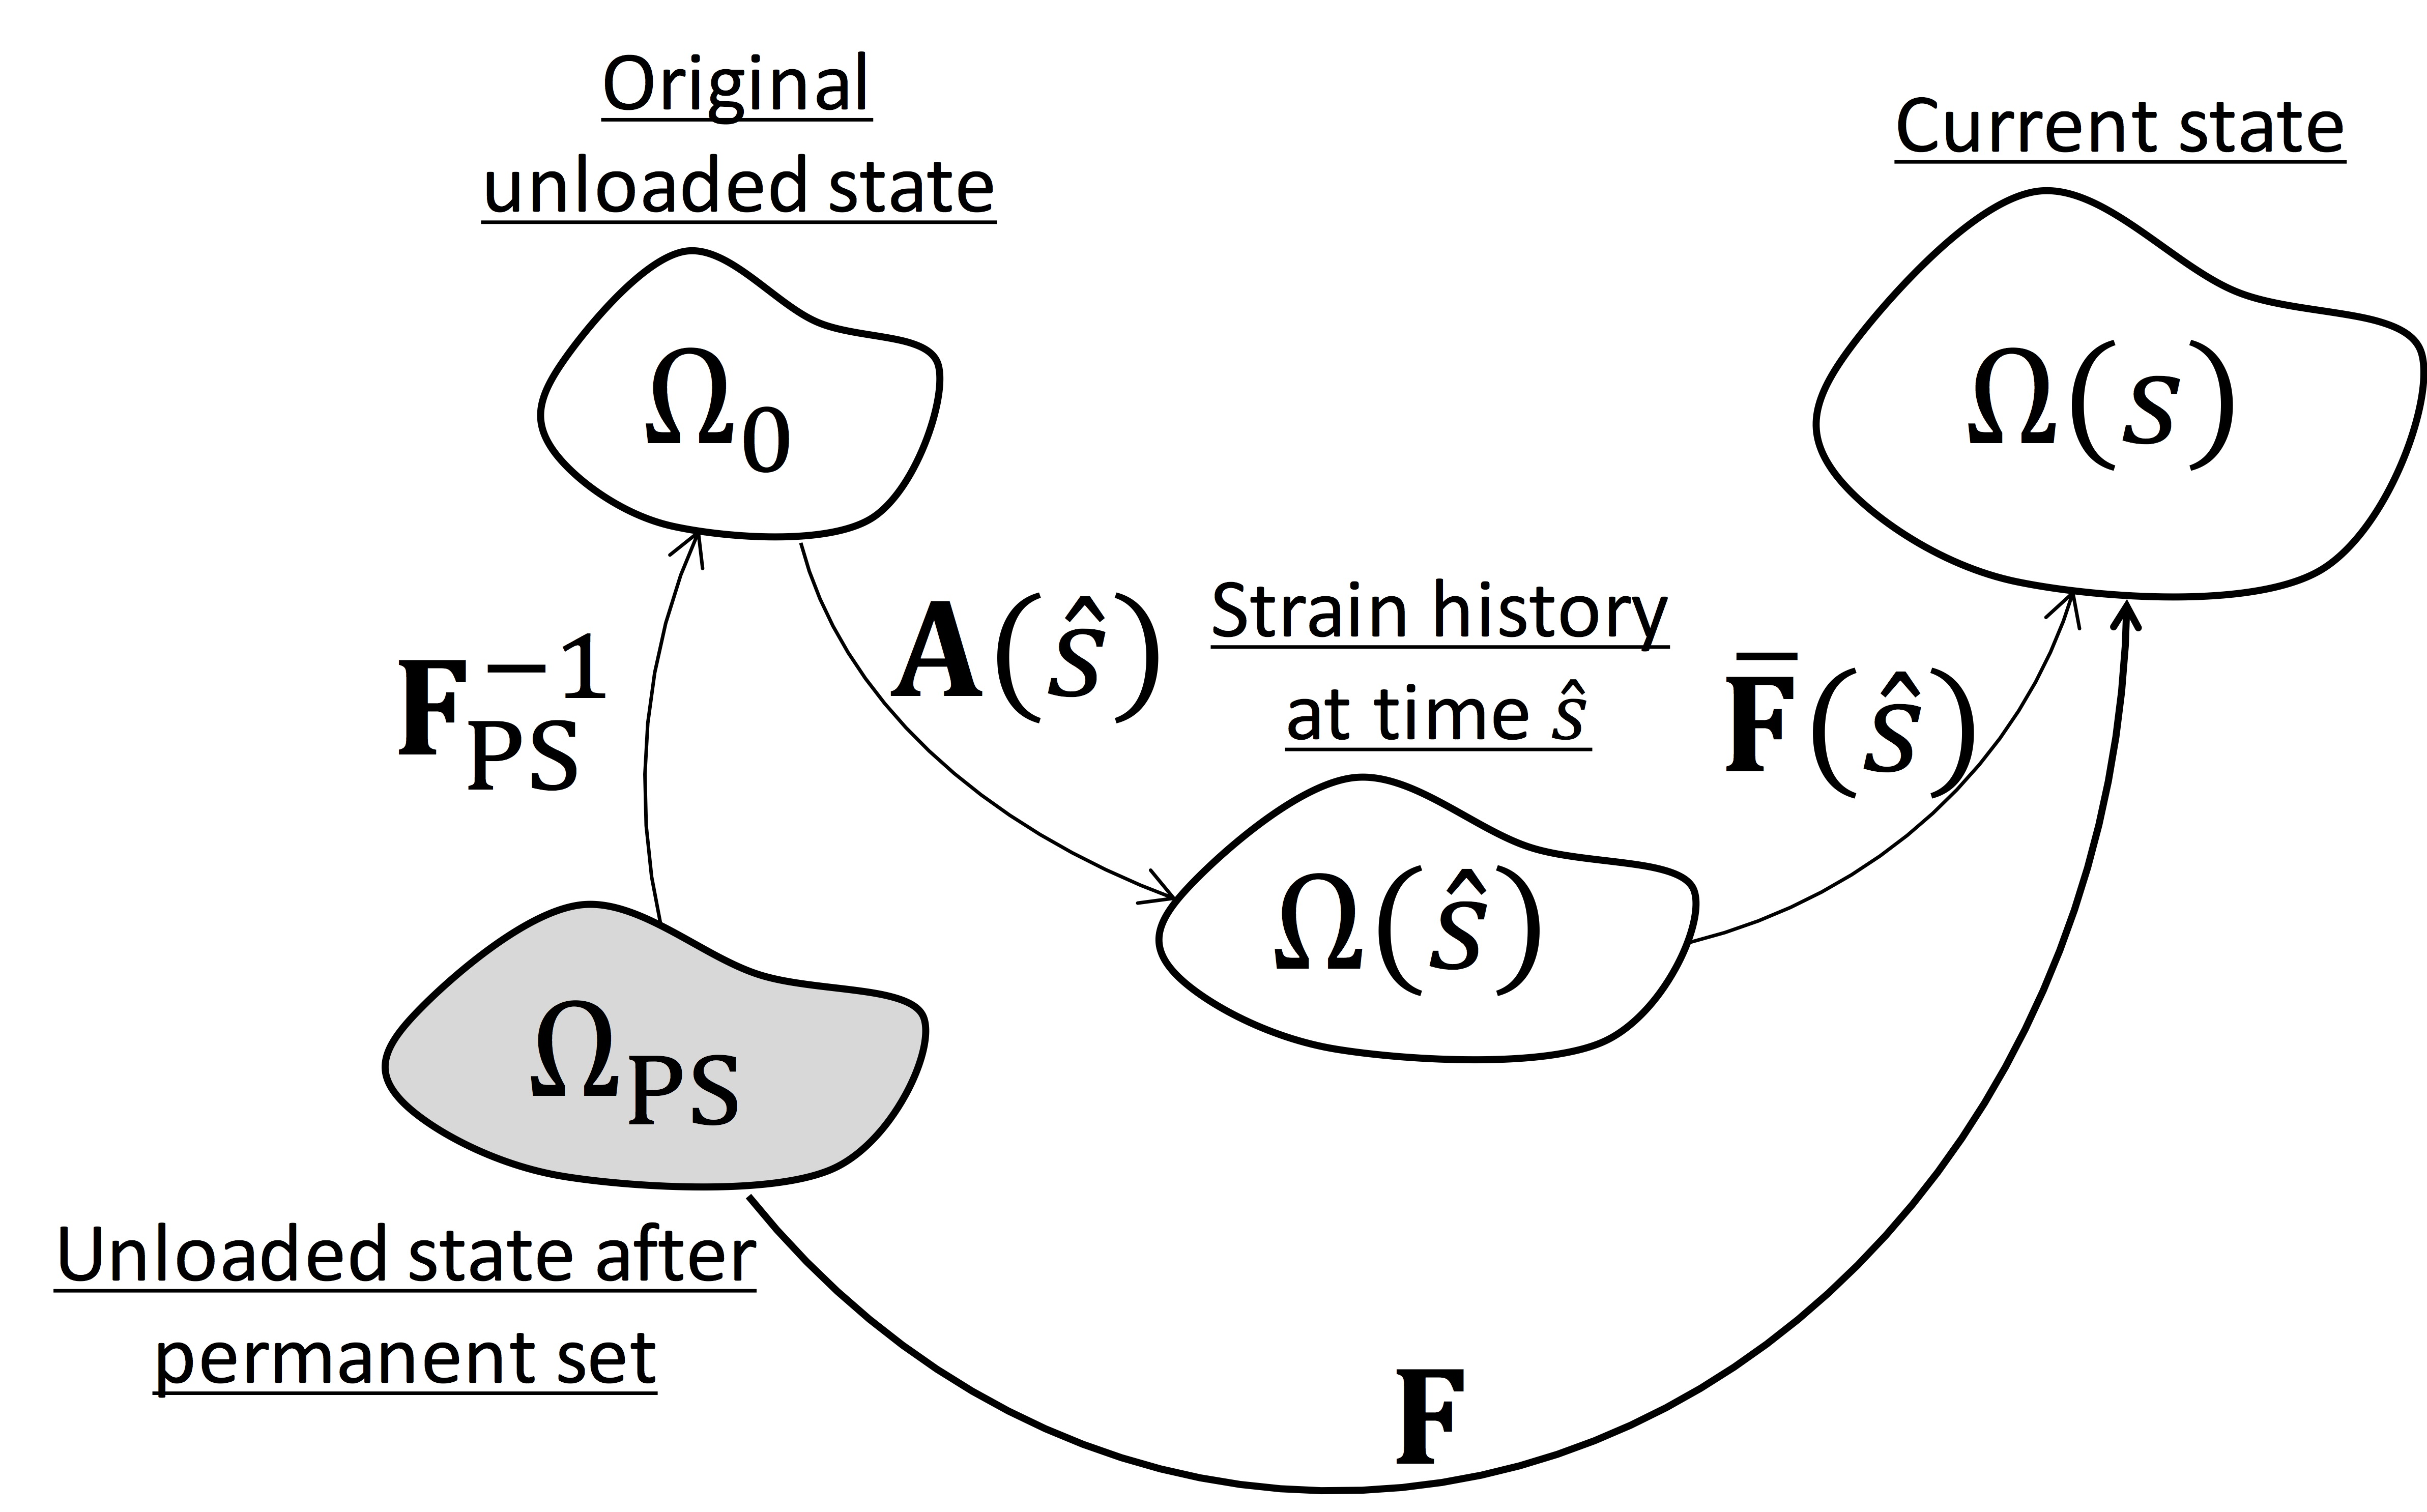
\includegraphics[width=4in]{Images/chapter4/figure8}
\caption{Modification of the relation between the different reference configurations when the unloaded configuration changes.}
\label{fig:PSevolution}
\end{figure}


%%%%%%%%%%%%%%%%%%%%%%%%%%%%%%%%%%%%%%%%%%%%%%%%%%%%%%%%%%%%%%%%%%%%%%%%%%%%%%%%
%%%%    Change in reference configuration

\subsection{Extension to the EXL matrix model for changes in reference configuration}

	We start by extending the EXL matrix model from our previous model \cite{sacks_novel_2016}. The strain energy is a modified form of the Yeoh model, which exhibits the following stress-strain relation,
\begin{equation}
\begin{split}
\Psi_m = &\frac{\eta_m}{2} \left( \frac{1}{\alpha}\left( I_1 -3\right)^{\alpha} + \frac{r}{\beta} \left( I_1 -3\right)^{\beta} \right), \\
&\text{with } 1<\alpha<\beta, \alpha\beta <2, 0 \leq r.
\end{split}
\end{equation}
    Here $\eta_m$ is the EXL matrix modulus, $\alpha,\beta$ are the exponent and $r$ is the relative weight between the two terms which is typically between 10 to 20. To modify the model form to reference the configuration at the time of formation $\Omega(\hat{s})$, we make the substitution for $\bar{I}_1(\mathbf{F}_\mathrm{PS}, \mathbf{A}(\hat{s}))$ (Eqn. \ref{eq:pseudo1stinv}),
\begin{equation} \label{eq:matrixenergyform}
\bar{\Psi}_m\left( \mathbf{C}, \mathbf{A}(\hat{s})\right) = \frac{\eta_m}{2} \left(\frac{1}{\alpha} \left( \bar{I}_1\left(\mathbf{F}_\mathrm{PS}, \mathbf{A}(s)\right) -3\right)^\alpha +\frac{r}{\beta} \left( \bar{I}_1\left(\mathbf{F}_\mathrm{PS}, \mathbf{A}(s)\right) -3\right)^\beta \right),
\end{equation}
    The derivative of the strain energy with respect to the invariant $\bar{I}_1$ is 
\begin{equation}
\frac{\partial \bar{\Psi}}{\partial \bar{I}_1} =	\frac{\eta_m}{2} \left(\left( \bar{I}_1\left(\mathbf{F}_\mathrm{PS}, \mathbf{A}(s)\right)- 3\right)^{\alpha - 1} + r \left( \bar{I}_1\left(\mathbf{F}_\mathrm{PS}, \mathbf{A}(s)\right) - 3\right)^{\beta - 1}\right).
\end{equation}
    After solving for the Lagrange multiplier $p$, with $\bar{S}_{m,33} = 0$, we have 
\begin{equation}\label{eq:matrixfinal}
\begin{split}
\mathbf{\bar{S}}_m \left( \mathbf{F}_\mathrm{PS},\mathbf{A}(\hat{s}),\mathbf{C}\right) &= \mu_m \left(\left( \bar{I}_1\left(\mathbf{F}_\mathrm{PS}, \mathbf{A}(s)\right) - 3\right)^{\alpha - 1} + r \left( \bar{I}_1\left(\mathbf{F}_\mathrm{PS}, \mathbf{A}(s)\right) - 3\right)^{\beta - 1}\right) \\
&\times \left( \mathbf{\tilde{B}}(\mathbf{F}_\mathrm{PS}, \mathbf{A}(\hat{s}))^{-1} - \tilde{B}_{33}^{-1}(\mathbf{F}_\mathrm{PS}, \mathbf{A}(\hat{s}))C_{33}\mathbf{C}^{-1}\right).
\end{split}
\end{equation}


%%%%%%%%%%%%%%%%%%%%%%%%%%%%%%%%%%%%%%%%%%%%%%%%%%%%%%%%%%%%
%%%%%%      Extension for permanent set

\subsubsection{Extension of the EXL matrix for the permanent set effect}

	Next, we developed the model form for the EXL matrix after permanent set. This approach is based on the work by Rajagopal and Wineman \cite{rajagopal_constitutive_1992}, where we assume that the response of the full EXL matrix to be 
\begin{equation} \label{eq:wineman}
\phi_m \mathbf{S}_m = b(s)\mathbf{\bar{S}}_m^\mathrm{existing} + \int\displaylimits_0^s a(s,\hat{s})\mathbf{\bar{S}}_m^\mathrm{new} \mathrm{d}\hat{s},
\end{equation}
    where $b(s)$ is the remaining amount of the existing material, $a(s,\hat{s})$ is the remaining amount of the new material formed during the strain history ($\mathbf{A}(s)$) at time $\hat{s}$, $\mathbf{\bar{S}}_m^\mathrm{existing}$ is the stress of the existing material and $\mathbf{\bar{S}}_m^\mathrm{new}$ is the stress of the new material. Assuming first order kinetics with the permanent set rate constant $k $, we have for the material remaining (Fig. \ref{fig:masstransfer})
\begin{equation}
\frac{\partial b(s)}{\partial s} = - k\cdot b(s), \qquad \frac{\partial a(s,\hat{s})}{\partial s} = - k \cdot a(s,\hat{s}).
\end{equation}
    Given that the total amount of EXL matrix ($\phi_m$) has not changed, $b(s) + \int_0^s a(s, \hat{s}) \mathrm{d}\hat{s} = \phi_m$, and we have
\begin{equation}
b(s) = \phi_m \mathrm{Exp}\left[-k  \cdot s\right], \qquad a(s,\hat{s}) = \phi_m k  \mathrm{Exp}\left[-k (s - \hat{s})\right].
\end{equation}
    Substitution into equation \ref{eq:wineman}, we have the mechanical response of the EXL matrix after permanent set,
\begin{equation}
\begin{aligned}
\phi_m \mathbf{S}_m =& \phi_m \left[\mathrm{Exp}\left[-k  \cdot s\right]\mathbf{\bar{S}}_m \left(\mathbf{F}_\mathrm{PS},\mathbf{A}(0),\mathbf{C}\right) \phantom{\int\displaylimits_0^s} \right. \\
&+ \left. \int\displaylimits_0^s k \cdot \mathrm{Exp}\left[-k (s - \hat{s})\right] \mathbf{\bar{S}}_m \left(\mathbf{F}_\mathrm{PS},  \mathbf{A}(\hat{s}),\mathbf{C}\right) \mathrm{d}\hat{s} \right].
\end{aligned}
\end{equation}
    The final form for the EXL matrix component of the permanent set model is thus,
\begin{equation}
\begin{split}
\phi_m \mathbf{S}_m &\left(\mathbf{F}_\mathrm{PS}, \mathbf{A}(\hat{s}),\mathbf{C}\right) \\
=& \phi_m \mu_m \left[ \vphantom{\int\displaylimits_0^s} \mathrm{Exp}\left[-k  \cdot s\right]  \left(\left( \bar{I_1} (\mathbf{F}_\mathrm{PS}, \mathbf{A}(0)) - 3\right)^{\alpha - 1} + r \left( \bar{I_1} (\mathbf{F}_\mathrm{PS}, \mathbf{A}(0)) - 3\right)^{\beta - 1}\right)  \right.\\
&\times \left( \mathbf{\tilde{B}}(\mathbf{F}_\mathrm{PS}, \mathbf{A}(0))^{-1} - \tilde{B}_{33}(\mathbf{F}_\mathrm{PS}, \mathbf{A}(0))^{-1}C_{33}\mathbf{C}^{-1}\right) \\
&+ \int\displaylimits_0^s k \cdot \mathrm{Exp}\left[-k (s - \hat{s})\right] \left(\left( \bar{I_1} (\mathbf{F}_\mathrm{PS}, \mathbf{A}(\hat{s})) - 3\right)^{\alpha - 1} + r \left( \bar{I_1} (\mathbf{F}_\mathrm{PS}, \mathbf{A}(\hat{s})) - 3\right)^{\beta - 1}\right) \\
&\times \left. \vphantom{\int\displaylimits_-^s} \left( \mathbf{\tilde{B}}(\mathbf{F}_\mathrm{PS}, \mathbf{A}(\hat{s}))^{-1} - \tilde{B}_{33}(\mathbf{F}_\mathrm{PS}, \mathbf{A}(\hat{s}))^{-1}C_{33}\mathbf{C}^{-1}\right) \mathrm{d}\hat{s}\right].
\end{split}
\end{equation}

\begin{figure}[hbt]
\centering
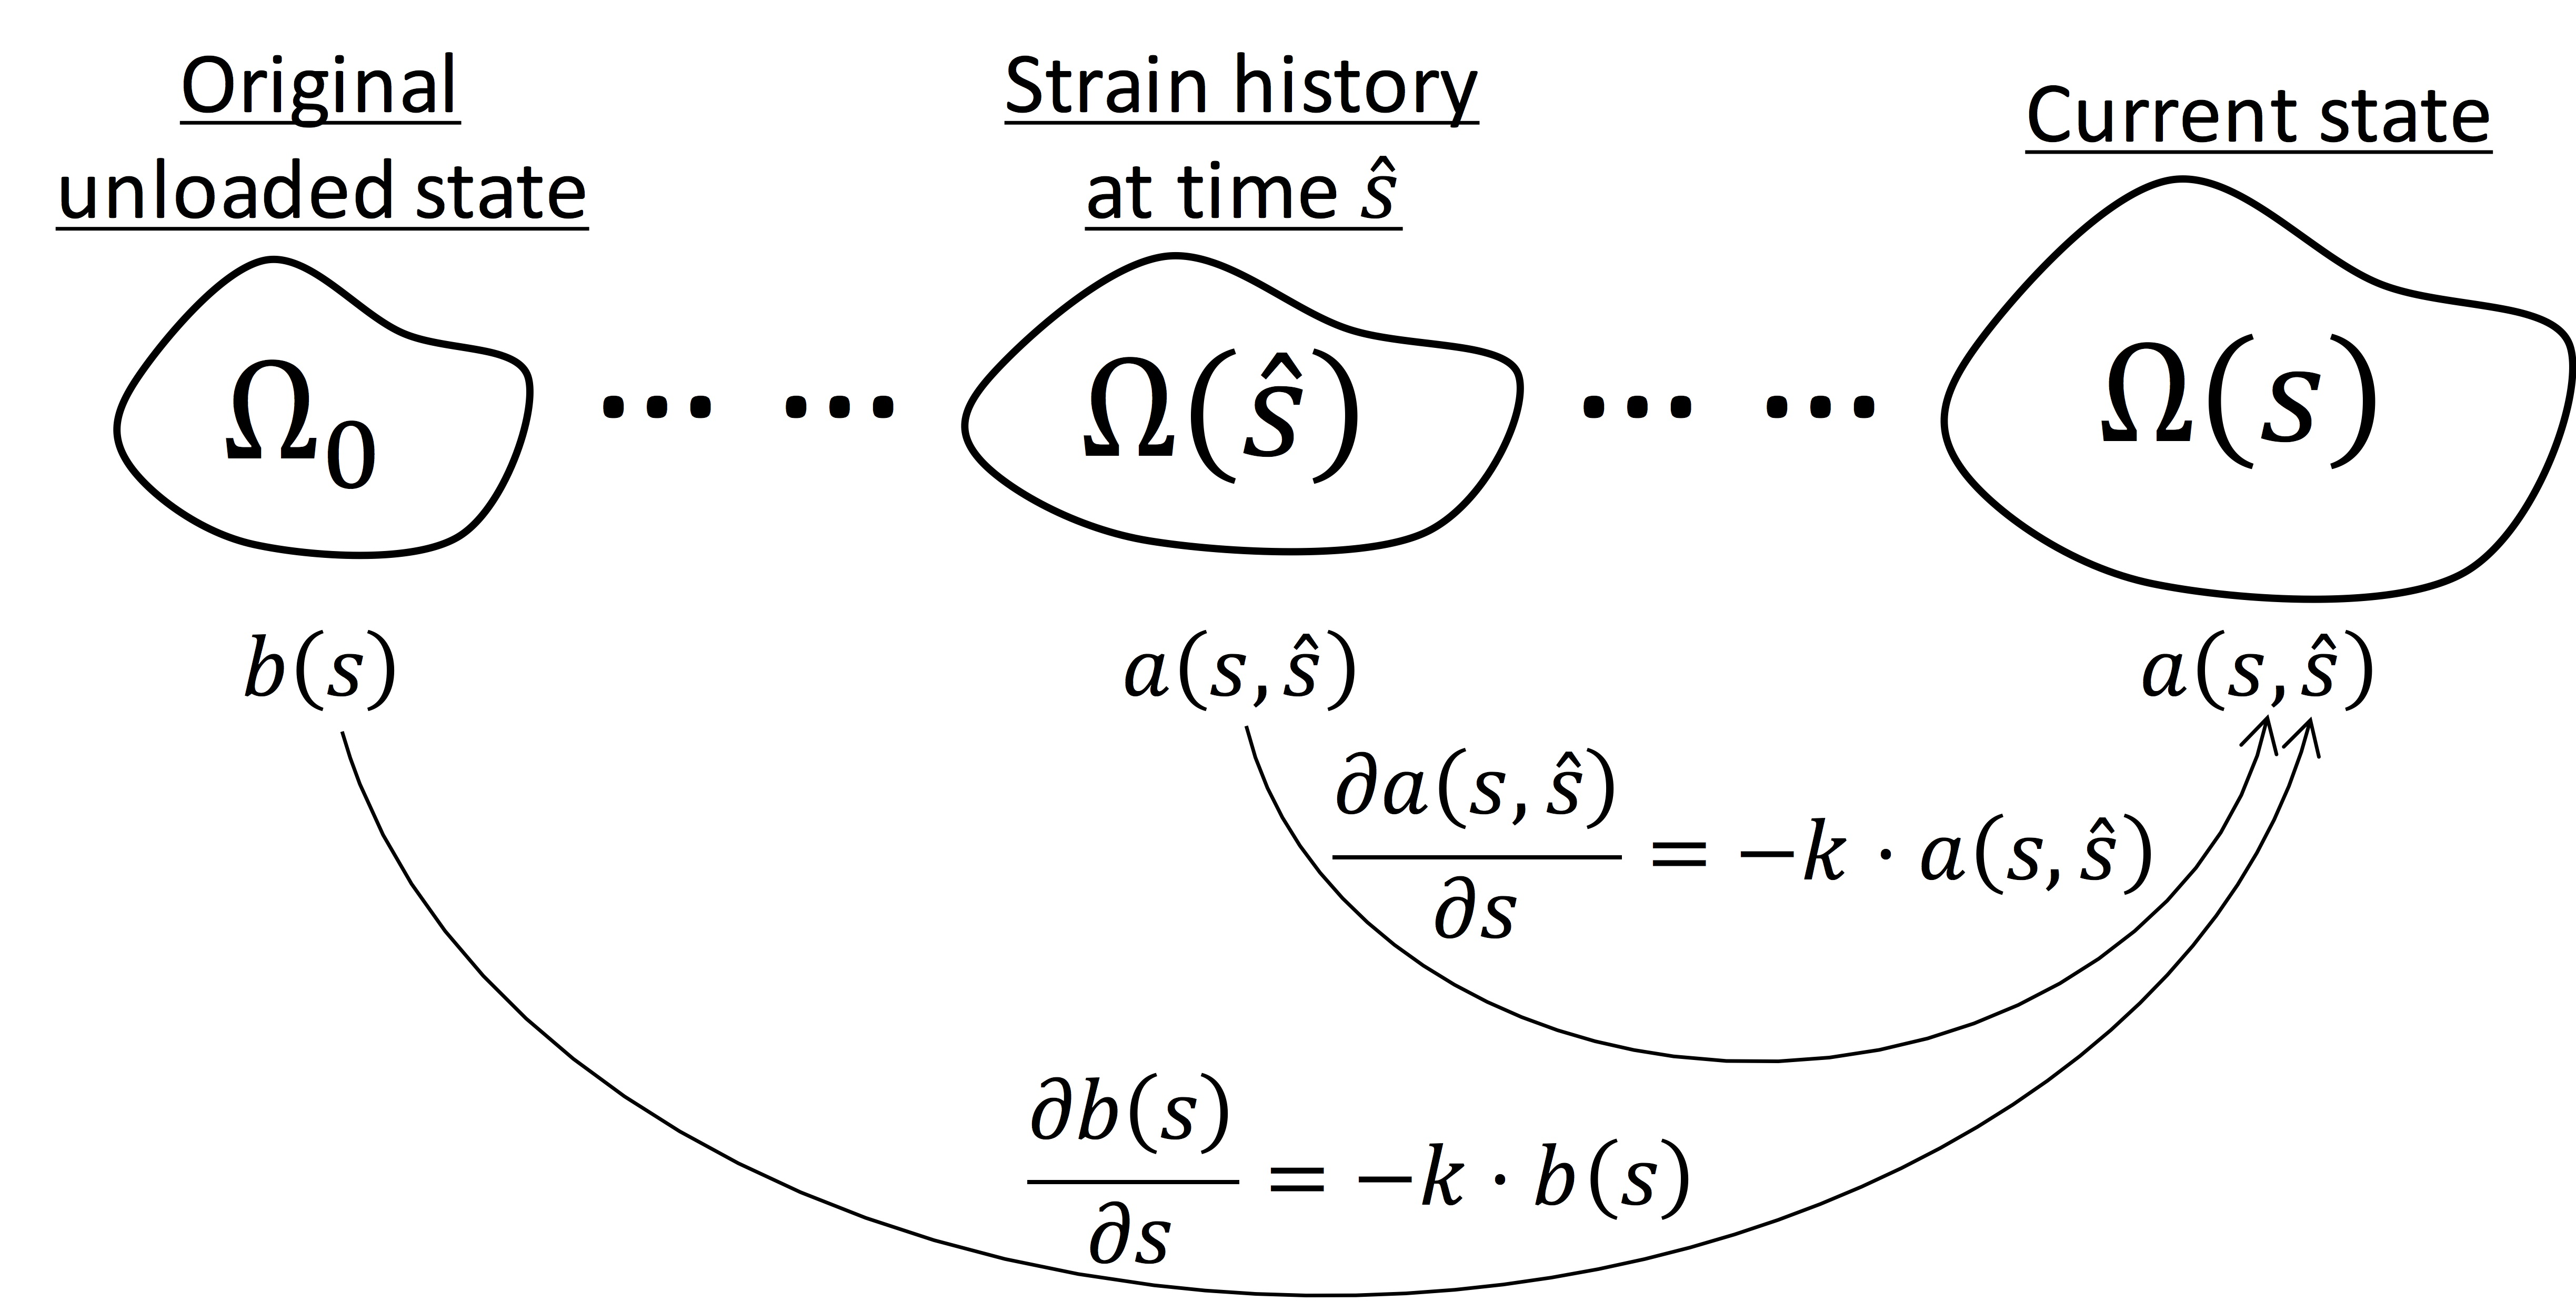
\includegraphics[width=4.5in]{Images/chapter4/figure9}
\caption{The mass fractions of the EXL matrix change over time, assuming first order kinetics. }
\label{fig:masstransfer}
\end{figure}

%%%%%%%%%%%%%%%%%%%%%%%%%%%%%%%%%%%%%%%%%%%%%%%%%%%%%%%%%%%%%%%%%%%%%%%%%%%%%%%%
%%%%    Structural Convection

\subsection{Convection of the collagen fiber architecture} \label{sec:convection}

    Now that the model form for the EXL matrix under permanent set is established, we need to consider how the collagen fiber architecture is convected by the change in reference configuration. The convection of the collagen fiber architecture is done through two parts: the ODF and the recruitment function. This is done by assuming that the collagen fiber architecture is convected under the affine assumption\cite{lee_presence_2015}. The form of the ODF and the recruitment distribution was previously described in Zhang \textit{et al.} \cite{zhang_meso_2016}, and the operation used to convect the collagen fiber architecture is given in Sacks \textit{et al}. \cite{sacks_novel_2016}. Briefly, the convected ODF $\Gamma_1$ is determined from the ODF in the 0-cycle state $\Gamma_0$ and the deformation $\prescript{1}{0}{\mathbf{F}}$ by the conservation of the number of fiber $\Gamma(\theta_0) \mathrm{d}\theta_0 = \Gamma(\theta_1) \mathrm{d}\theta_1$ (Fig. \ref{fig:effectsofconvection}A). This is given by
\begin{equation} \label{eq:pfODF}
\begin{gathered}
\Gamma_1\left( \prescript{1}{0}{\mathbf{F}},\theta_1 \right) = \Gamma_0\left( \theta_0\left( \prescript{1}{0}{\mathbf{F}},\theta_1\right)\right)\frac{\prescript{1}{0}{\lambda(\theta_0)}^2}{\prescript{1}{0}{J_\mathrm{2D}}}, \\
\prescript{1}{0}{\lambda(\theta_0)} = \sqrt{\mathbf{n}_{\theta_0}\cdot  \prescript{1}{0}{\mathbf{F}^\mathsf{T}}  \prescript{1}{0}{\mathbf{F}} \cdot \mathbf{n}_{\theta_0}}, \qquad \prescript{1}{0}{J_\mathrm{2D}} =\det (\prescript{1}{0}{\mathbf{F}}),
\end{gathered}
\end{equation}
    where $\mathbf{n}_\theta$ is a unit vector for the orientation $\theta$. The distribution of slack stretch needed to straighten collagen fiber crimp after convection, in other words the recruitment distribution $D_1(\lambda_s)$ (Fig. \ref{fig:effectsofconvection}B), is given by
\begin{equation} \label{eq:pfrecruitment}
\begin{gathered}
D_1(\prescript{1}{0}{\mathbf{F}}, \lambda_s) = \begin{cases} \frac{\operatorname{B}[\gamma_0,\gamma_1](y)}{\prescript{}{1}{\lambda}_\mathrm{ub}-\prescript{}{1}{\lambda}_\mathrm{lb}} & \prescript{}{1}{\lambda}_\mathrm{ub} < y < \prescript{}{1}{\lambda}_\mathrm{lb} \\ 0 & \text{else}\end{cases}, \\
\qquad \prescript{}{1}{\lambda}_s = \frac{\lambda_s}{\prescript{1}{0}{\lambda}(\theta)}, \qquad y = \frac{\prescript{}{1}{\lambda}_s - \prescript{}{1}{\lambda}_\mathrm{lb}}{\prescript{}{1}{\lambda}_\mathrm{ub}-\prescript{}{1}{\lambda}_\mathrm{lb}}.
\end{gathered}
\end{equation}
where $\prescript{1}{0}{\lambda(\theta_0)}$ is defined in equation \ref{eq:pfODF}, $(\prescript{}{1}{\lambda}_\mathrm{lb},\prescript{}{1}{\lambda}_\mathrm{ub})$ are the new bounds of the distribution after being convected, and $(\gamma_0,\gamma_1)$ are the shape parameters of the beta distribution function $B$ .
The model form for collagen fibers in exogenously crosslinked BP after being convected by a change in geometry is previously presented in Sacks et al. \cite{sacks_novel_2016} and can also be used for the convection of the collagen fiber architecture due to the permanent set effect. 
The model form for the fiber ensemble interactions is given by equation \ref{eq:interaction}, where equations \ref{eq:pfODF} and \ref{eq:pfrecruitment} are substituted in for the ODF and recruitment distribution function for the mechanical response after permanent set.


\begin{figure}[hbt]
\centering
\centerline{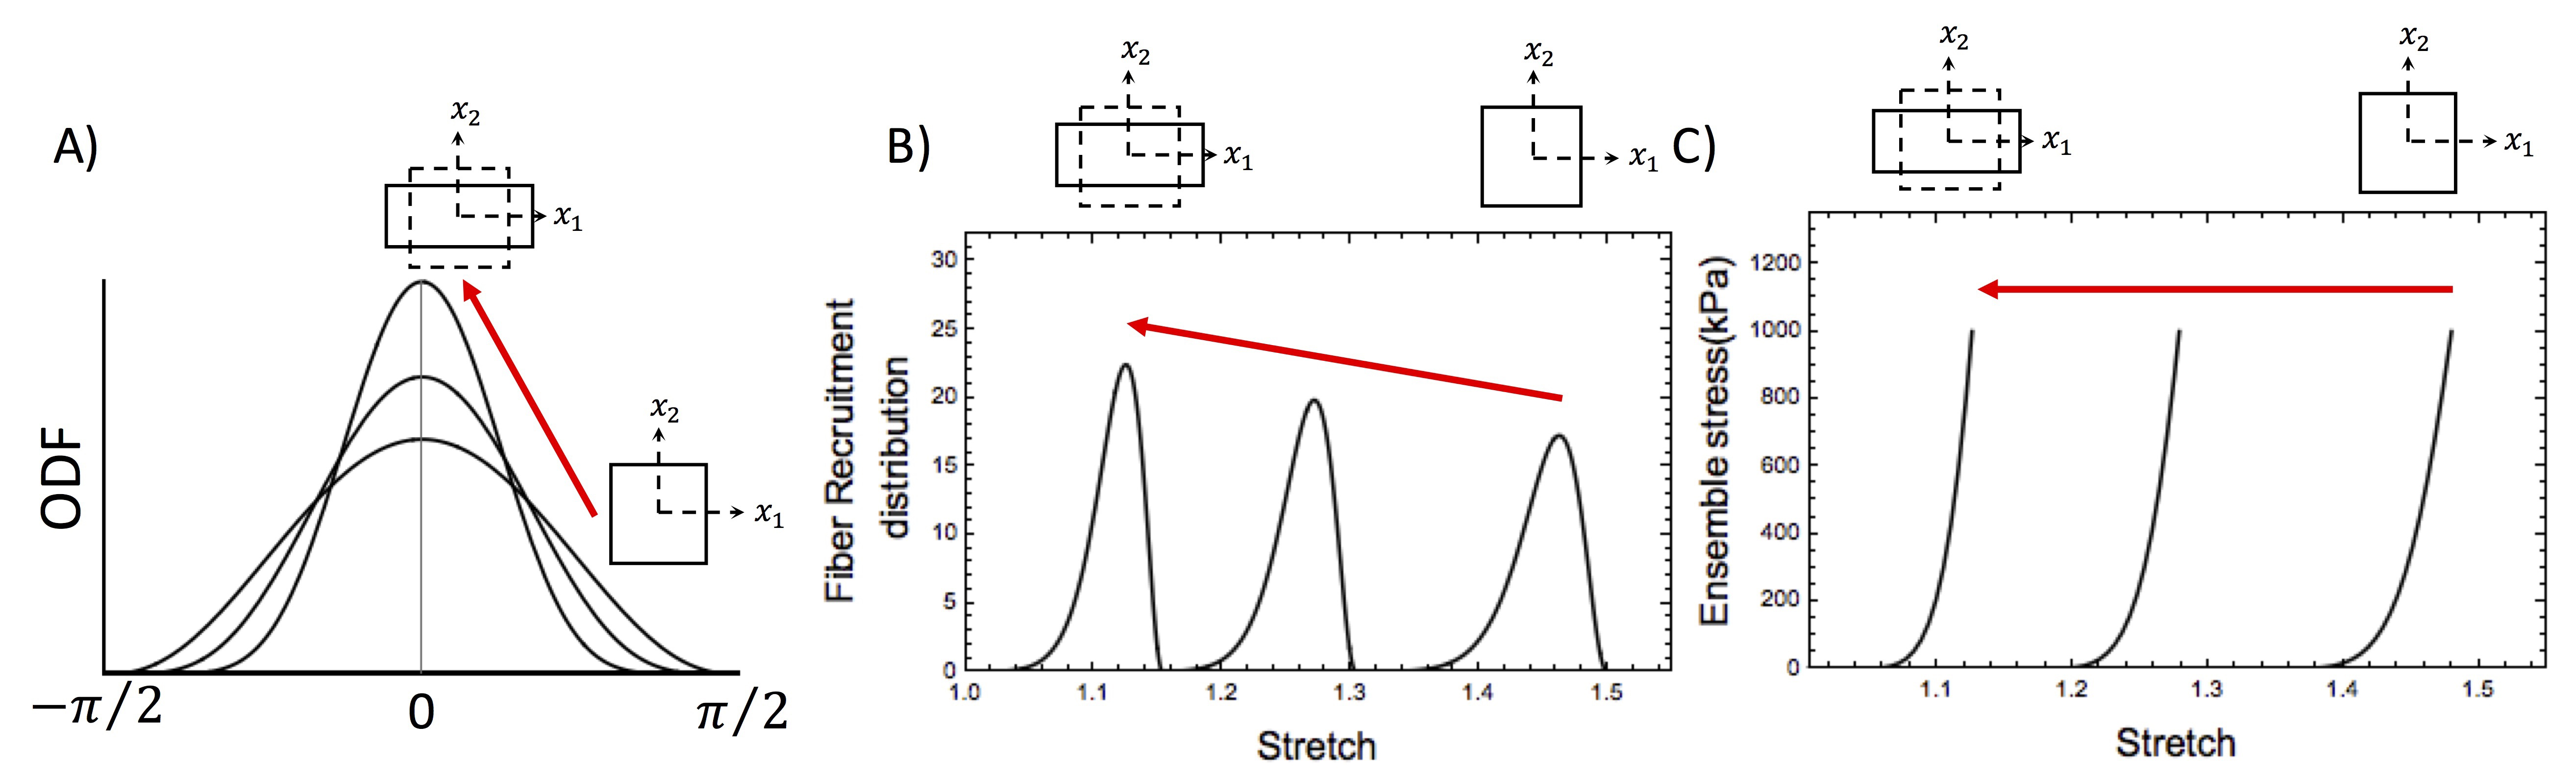
\includegraphics[width=\textwidth]{Images/chapter4/figure10}}
\caption{The effects of convecting the collagen fiber architecture show A) gradual alignment of collagen fibers, B) changes in the probability distribution of collagen fiber lack stretches and C) its effect on the mechanical response.}
\label{fig:effectsofconvection}
\end{figure}



%%%%%%%%%%%%%%%%%%%%%%%%%%%%%%%%%%%%%%%%%%%%%%%%%%%%%%%%%%%%%%%%%%%%%%%%%%%%%%%%
%%%%    Further considerations

\subsection{Further considerations of the permanent set mechanism.}

	In addition to the above considerations, we explored the the following as a means to validate the mechanisms we proposed for permanent set. This was done by performing an analysis on predicting the mechanical response after cyclic loading using only the convection of the collagen fiber architecture by the measured $\textbf{F}_{PS}$. The analysis takes the following steps: 1) Material model parameter estimation for the 0-cycle data for the strain controlled data. This is done using the approach from Sacks \textit{et al}.\cite{sacks_novel_2016}, with the constitutive model for collagen fibers and the EXL matrix from the same study, and the interaction model from equation \ref{eq:interaction}. 
	2) Use equations \ref{eq:pfODF} and \ref{eq:pfrecruitment} (Sec.\ref{sec:convection}) to convect the collagen fiber architecture (Fig. \ref{fig:structuralconvection} and Fig. \ref{fig:effectsofconvection}). 
	The deformation used to convect the collagen fiber architecture is determined from the fiducial markers. 
	3) We compare the new convected exogenously crosslinked mechanical response to the experimental data.

%\subsection{Mechanical response predicted from convected collagen fiber architecture vs experimental data after cycling}

	We used this approach to examine both the strain (n = 3) and stress controlled specimens (n = 5), and tested the hypothesis that \emph{there is a significant different between the mechanical response predicted from structural convection and the experimentally measure data}, in other words, our model is not sufficient to explain the change in mechanical response. We take the maximum stress of each specimen under equibiaxial strain, and compared the difference between the model and the experimental data using student t-test.	For the strain control specimens, we found that there is no statistical significant difference between the convected mechanical response and the experimental data, where the average p-value of the PD and XD for both after 30 million cycle and after 65 million cycle is $p = 0.37$ (minimum $p > 0.07$). 
	Likewise, we also found no statistical significant differences between the convected response and the experimental data for the stress controlled specimens, where the average p-value is 0.57 (Fig. \ref{fig:mechconvec}).
	These results suggest that 1) the underlying collagen fiber architecture, including collagen fiber crimp and orientation, is convected affinely according to the permanent set in the EXL matrix. This indicates that our approach to model permanent set is realistic, and the underlying mechanism for permanent set is likely to be correct. 
	2) Structural damage to the collagen fiber architecture was not detectable at this stage (up to 65 million cycles). 
	These important results indicate that permanent set alone is sufficient to capture the response to cyclic loading up to 50-65 million cycles. 


\begin{figure}[hbt]
\centering
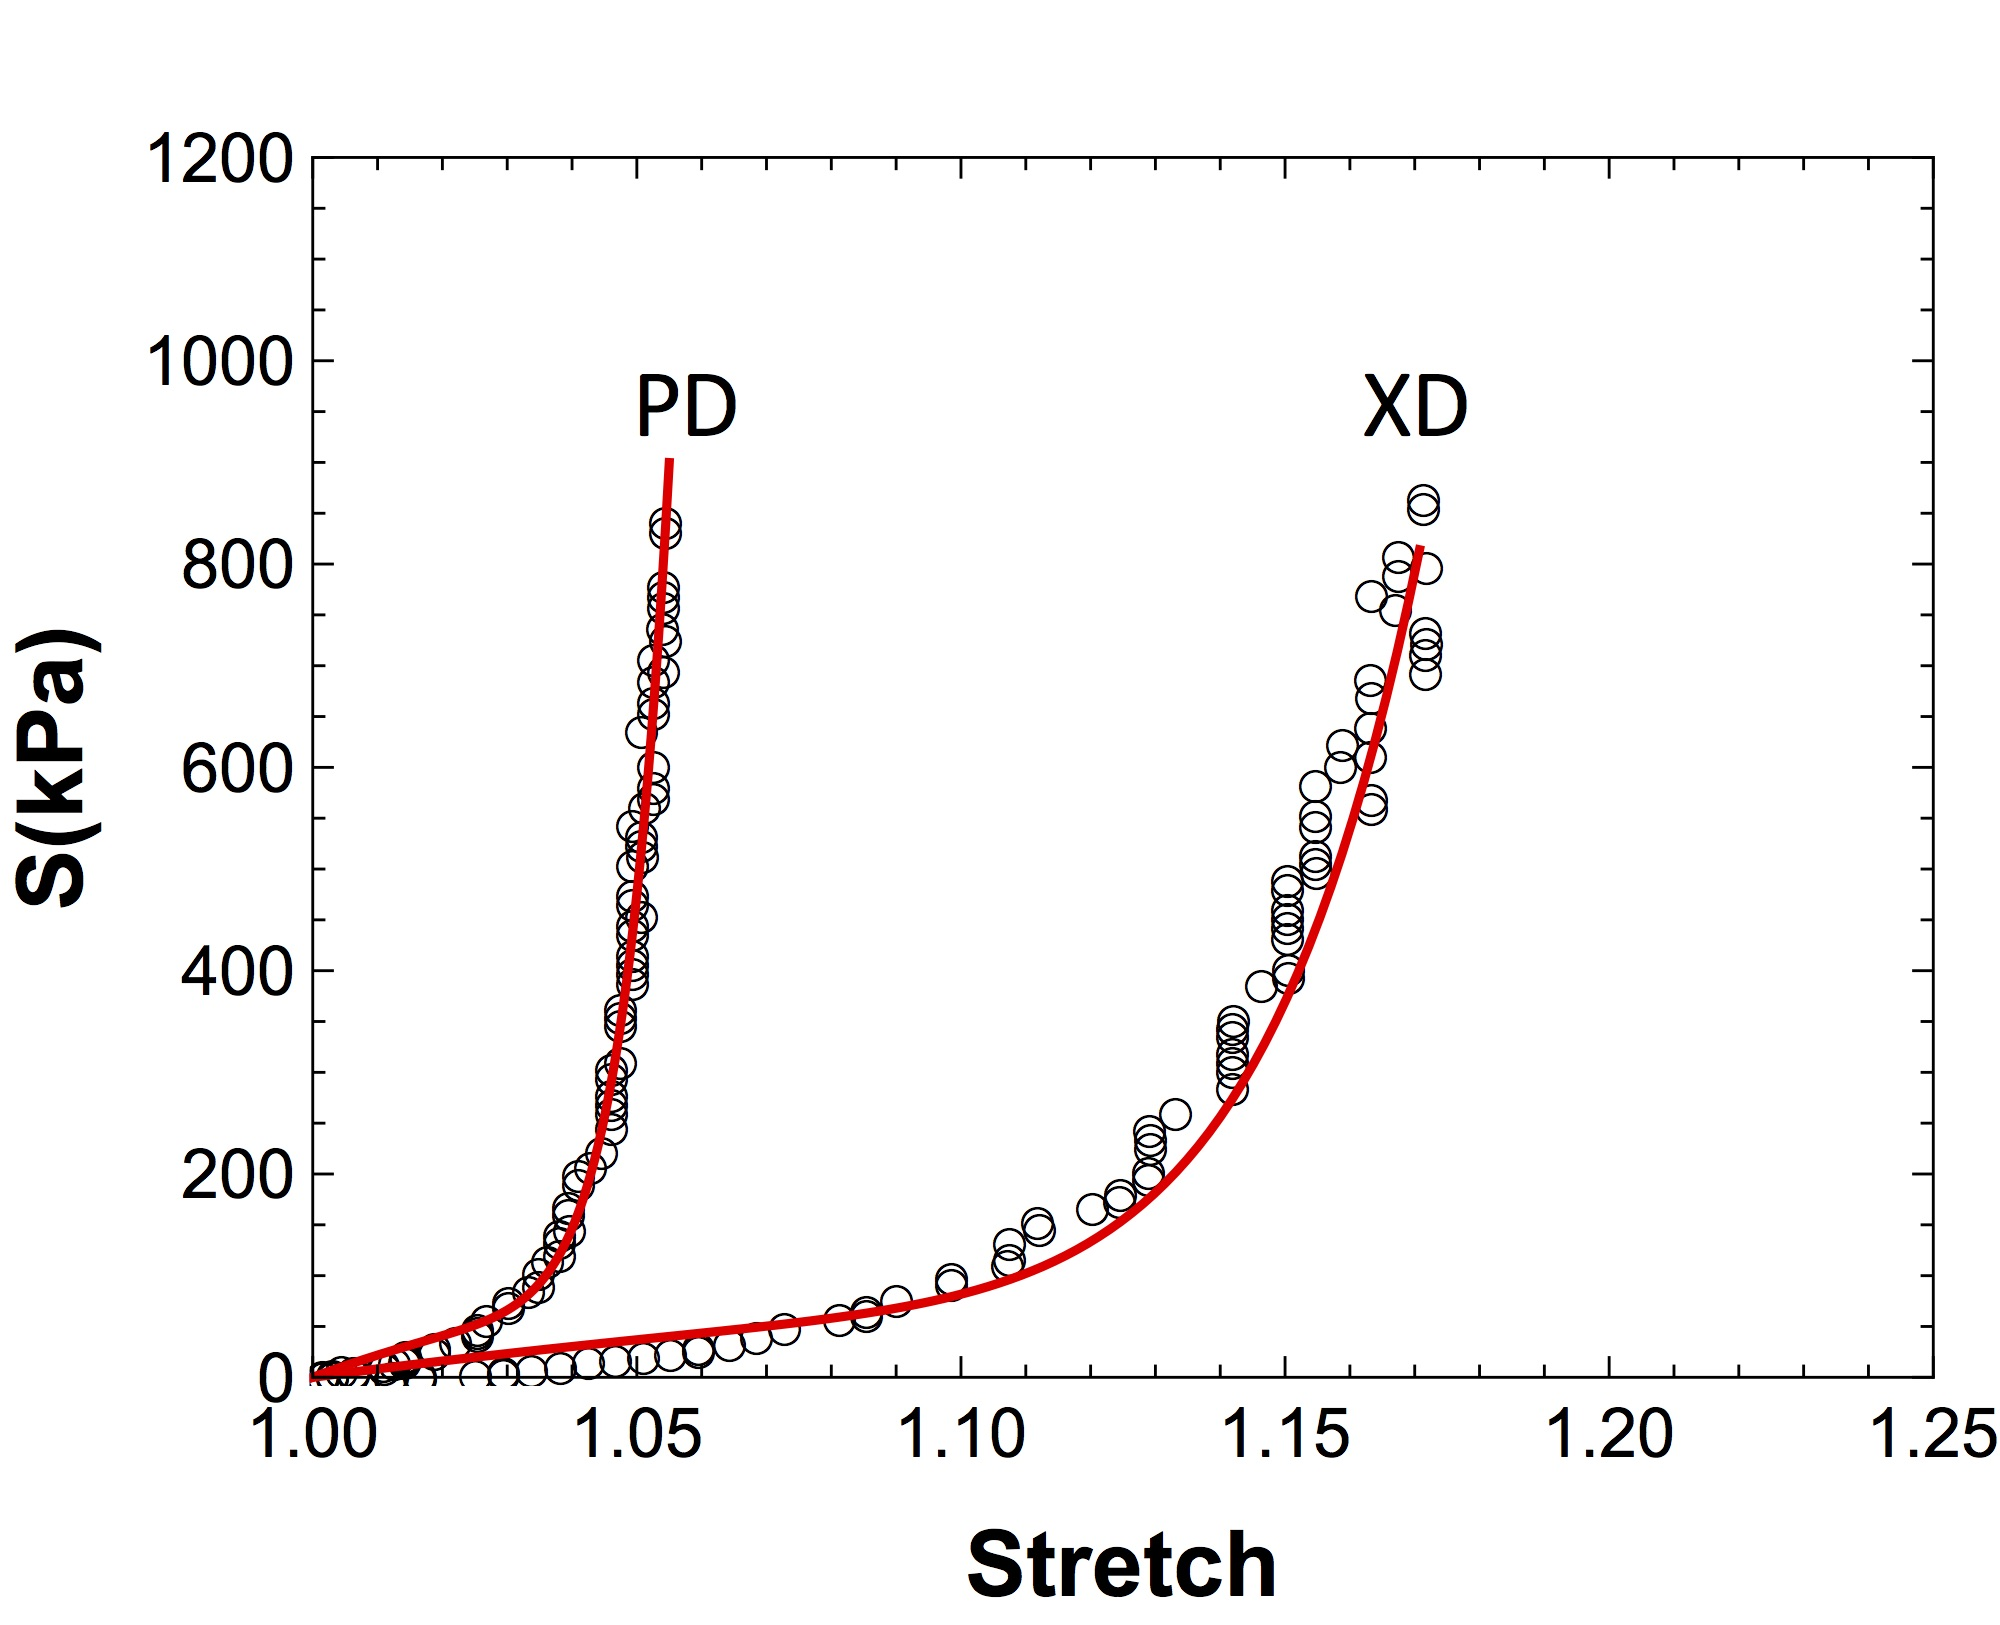
\includegraphics[width=3.5in]{Images/chapter4/figure11}
\caption{The equibiaxial mechanical response of an exogenously crosslinked BP specimen after 50 million cycles and the mechanical response determined from structural convection (Red) using the measured $\textbf{F}_{PS}$}
\label{fig:mechconvec}
\end{figure}


%%%%%%%%%%%%%%%%%%%%%%%%%%%%%%%%%%%%%%%%%%%%%%%%%%%%%%%%%%%%%%%%%%%%%%%%%%%%%%%%
%%%%    Full model form

\subsection{Full model form}
	Combining all three components, we have the final model form as a function of the permanent set rate constant $k $, the permanent set deformation $\mathbf{F}_\mathrm{PS}$, the strain history $\mathbf{A}(s)$, and the material parameters of the constitutive model in the uncycled state. The input of the model is the applied deformation $\mathbf{C}$ referenced to the current unloaded state $\Omega_\mathrm{PS}$, given by the deformation $\mathbf{F}_\mathrm{PS}$ from $\Omega_0$. The full form is
\begin{equation}\label{eq:fullEXLmodel}
\mathbf{S} = \mathbf{S}\left(k , \mathbf{F}_\mathrm{PS}, \mathbf{A}(\hat{s}), \mathbf{C}\right) = \phi_\mathrm{col} \left[ \mathbf{S}_\mathrm{col} + \mathbf{S}_\mathrm{int}\right] + \phi_m \mathbf{S}_\mathrm{m},
\end{equation}
where the collagen contribution is 
\begin{equation} \label{eq:fullcollagen}
\begin{split}
\phi_\mathrm{col}\mathbf{S}_\mathrm{col}&\left(k , \mathbf{F}_\mathrm{PS}, \mathbf{A}(\hat{s}), \mathbf{C}\right) \\
&= \phi_\mathrm{col} \eta_C \int\displaylimits_\theta \Gamma_1(\mathbf{F}_{\mathrm{PS}}, \theta)\left\lbrace 
\int\displaylimits_1^{\lambda_\theta} \frac{D_1\left( \mathbf{F}_{\mathrm{PS}}, x \right)}{x} \left( \frac{1}{x}- \frac{1}{\lambda_\theta}\right) \mathrm{d}x \right\rbrace \mathbf{n}_\theta\otimes\mathbf{n}_\theta \mathrm{d}\theta,
\end{split}
\end{equation}
where $\lambda_\theta = \sqrt{\mathbf{n}_\theta \cdot \mathbf{C}\mathbf{n}_\theta}$ is the stretch of the fiber ensemble oriented along $\theta$, the fiber ensemble interactions is 
\begin{equation} \label{eq:fullinteractions}
\begin{split}
\phi_\mathrm{int}\mathbf{S}_\mathrm{int}&\left(k , \mathbf{F}_\mathrm{PS}, \mathbf{A}(\hat{s}), \mathbf{C}\right) \\
=& \phi_\mathrm{col} \eta_\mathrm{int} \int\displaylimits_\alpha \int\displaylimits_\beta \Gamma_1 \left(\mathbf{F}_\mathrm{PS}, \alpha \right) \Gamma_1 \left(\mathbf{F}_\mathrm{PS},  \beta \right) \\
&\times\left[ \left\lbrace 
\int\displaylimits_1^{\lambda_\alpha} \int\displaylimits_1^{\lambda_\beta} 
\frac{2 \lambda_\beta D_1(\mathbf{F}_\mathrm{PS}, x_\alpha) D_1(\mathbf{F}_\mathrm{PS}, x_\beta)}{x_\alpha x_\beta} 
\left( \frac{\lambda_\alpha}{x_\alpha} \frac{\lambda_\beta}{x_\beta} - 1\right) \mathrm{d}x_\alpha \, \mathrm{d}x_\beta \right.\right. \\
&+ \left. \left. \int\displaylimits_1^{\lambda_\beta} D_1(\mathbf{F}_\mathrm{PS}, x_\beta) \left( \frac{\lambda_\beta}{x_\beta} -1  \right)^2 \mathrm{d}x_\beta \right\rbrace \right.  \frac{\mathbf{n}_\alpha \otimes \mathbf{n}_\alpha}{\lambda_\alpha}  \\
&+ \left. \left\lbrace
\int\displaylimits_1^{\lambda_\alpha} \int\displaylimits_1^{\lambda_\alpha} 
\frac{2 \lambda_\beta D_1(\mathbf{F}_\mathrm{PS}, x_\alpha) D_1(\mathbf{F}_\mathrm{PS}, x_\beta)}{x_\alpha x_\beta} 
\left( \frac{\lambda_\alpha}{x_\alpha} \frac{\lambda_\beta}{x_\beta} - 1\right) \mathrm{d}x_\alpha \, \mathrm{d}x_\beta 
\right. \right. \\
&+\left. \left. \int\displaylimits_1^{\lambda_\alpha} D_1(\mathbf{F}_\mathrm{PS}, x_\alpha) \left( \frac{\lambda_\alpha}{x_\alpha} -1  \right)^2 \mathrm{d}x_\alpha \right\rbrace \frac{\mathbf{n}_\beta \otimes \mathbf{n}_\beta}{\lambda_\beta}  \right] \mathrm{d}\alpha \, \mathrm{d}\beta,
\end{split}
\end{equation}
and the EXL matrix is
\begin{equation} \label{eq:fullmatrix}
\begin{split}
\phi_m \mathbf{S}_\mathrm{m}&\left(k , \mathbf{F}_\mathrm{PS}, \mathbf{A}(\hat{s}), \mathbf{C}\right) \\
&= \phi_m \eta_m \left[ \vphantom{\int\displaylimits_0^s} \mathrm{Exp}\left[-k  \cdot s\right]  \left(\left( \bar{I_1} (\mathbf{F}_\mathrm{PS}, \mathbf{A}(0)) - 3\right)^{\alpha - 1} + r \left( \bar{I_1} (\mathbf{F}_\mathrm{PS}, \mathbf{A}(0)) - 3\right)^{\beta - 1}\right)  \right.\\
&\times \left( \mathbf{\tilde{B}}(\mathbf{F}_\mathrm{PS}, \mathbf{A}(0))^{-1} - \tilde{B}_{33}^{-1}(\mathbf{F}_\mathrm{PS}, \mathbf{A}(0))C_{33}\mathbf{C}^{-1}\right) \\
&+ \int\displaylimits_0^s k \cdot \mathrm{Exp}\left[-k (s - \hat{s})\right] \left(\left( \bar{I_1} (\mathbf{F}_\mathrm{PS}, \mathbf{A}(\hat{s})) - 3\right)^{\alpha - 1} + r \left( \bar{I_1} (\mathbf{F}_\mathrm{PS}, \mathbf{A}(\hat{s})) - 3\right)^{\beta - 1}\right) \\
&\times \left. \vphantom{\int\displaylimits_-^s} \left( \mathbf{\tilde{B}}(\mathbf{F}_\mathrm{PS}, \mathbf{A}(\hat{s}))^{-1} - \tilde{B}_{33}^{-1}(\mathbf{F}_\mathrm{PS}, \mathbf{A}(\hat{s}))C_{33}\mathbf{C}^{-1}\right) \mathrm{d}\hat{s}\right].
\end{split}
\end{equation}

%%%%%%%%%%%%%%%%%%%%%%%%%%%%%%%%%%%%%%%%%%%%%%%%%%%%%%%%%%%%%%%%%%%%%%%%%%%%%%%%
%%%%    Finding permanent set deformations

\subsection{Determining permanent set deformation and loaded state}
To solve for the permanent set deformation ($\mathbf{F}_\mathrm{PS}$), and for the deformation ($\mathbf{A}(s)$) to the new loaded state after permanent set ($\Omega(s)$) when under an applied stress of $\mathbf{\hat{S}}$, we need to use optimization as the permanent set constitutive model has no analytical inverse form. Specifically,
\begin{equation}\label{eq:optimization}
\begin{gathered}
\mathbf{F}_\mathrm{PS} = \operatorname*{arg\,min}_\mathbf{F} \left\Vert \mathbf{S}\left(k , \mathbf{I}, \mathbf{A}(\hat{s}), \mathbf{C}=\mathbf{F}^\mathsf{T}\mathbf{F}\right) - 0 \right\Vert, \\
\mathbf{A}(s) = \operatorname*{arg\,min}_\mathbf{F} \left\Vert \mathbf{S}\left(k , \mathbf{I}, \mathbf{A}(\hat{s}), \mathbf{C}=\mathbf{F}^\mathsf{T}\mathbf{F}\right) - \mathbf{\hat{S}} \right\Vert.
\end{gathered}
\end{equation}

%%%%%%%%%%%%%%%%%%%%%%%%%%%%%%%%%%%%%%%%%%%%%%%%%%%%%%%%%%%%%%%%%%%%%%%%%%%%%%%%
%%%%    Modeling and parameter estimation

\subsection{Modeling approach and parameter estimation}

%%%%%%%%%%%%%%%%%%%%%%%%%%%%%%%%%%%%%%%%%%%%%%%%%%%%%%%%%%%%
%%%%    Strain controlled cycling

\subsubsection{Strain controlled cycling}
	Our goal using the strain controlled data is to validate the constitutive model form and perform parameter estimation. Since the loaded state never changes, the permanent set model can be simplified into a two-state model, with the loaded state ($\Omega(s)$) being the root mean square strain. Specifically, the EXL matrix can be simplified to
\begin{equation} 
\begin{split}
\phi_m \mathbf{S}_m &= \phi_m \left[ \mathrm{Exp}\left[-k  \cdot s\right] \mathbf{\bar{S}}_m \left(\mathbf{F}_\mathrm{PS}, \mathbf{I},\mathbf{C}\right) + \int\displaylimits_0^s k \cdot  \mathrm{Exp}\left[-k (s - \hat{s})\right] \mathbf{\bar{S}}_m \left(\mathbf{F}_\mathrm{PS}, \mathbf{A},\mathbf{C}\right) \mathrm{d}\hat{s} \right] \\
&= \phi_m \left[ \mathrm{Exp}\left[-k  \cdot s\right] \mathbf{\bar{S}}_m \left(\mathbf{F}_\mathrm{PS}, \mathbf{I},\mathbf{C}\right) + \left(1 - \mathrm{Exp}\left[-k  \cdot s\right] \right) \mathbf{\bar{S}}_m \left(\mathbf{F}_\mathrm{PS}, \mathbf{A},\mathbf{C}\right) \right].
\end{split}
\end{equation}
Of the 3 time points (0, 30, and 65 million cycles), we fit the first two time points (0 and 30 million cycles) and use the results to predict the response to cycling at 65 million cycles as a way to validate our model (Fig. \ref{fig:datamethods}A). We note that the mounted configuration of the specimen for mechanical testing and cyclic loading are not the same, thus there is a small rigid body rotation of the specimen between the two testing configurations. We will compensate for this during the parameter estimation, which is done as followed
\begin{enumerate}
\item Determine the 0-cycled mechanical response using the methods of Sacks \textit{et al}.\cite{sacks_novel_2016}
\item Fit the permanent set deformation $\mathbf{F}_\mathrm{PS}$ and the mechanical response at the same time for the 30 million cycles time point
	\begin{enumerate}
	\item choose a $k $
	\item choose a mounting direction $\theta_\mathrm{mount}$
	\item compute $err_\mathrm{PS} = \mathbf{F}_\mathrm{PS} - \mathbf{F}_\mathrm{PS}^\mathrm{data}$ error at 30 million cycles
	\item compute $err_\mathrm{\mathbf{S}} = \mathbf{S}^\mathrm{max} - \mathbf{S}_\mathrm{data}^\mathrm{max}$
	\item compute the weighted error $err_\mathrm{PS} + W_\mathbf{S} err_\mathbf{S}$, where the weight $W_\mathbf{S} = $max strain in the direction of loading/$\mathbf{S}_\mathrm{data}^\mathrm{max}$
	\item update $k $ and $\theta_\mathrm{mount}$ using the Quasi-Newton method \cite{king_dlib_2009}
	\end{enumerate}
\item Predict $\mathbf{F}_\mathrm{PS}$ and the mechanical response at 65 million cycles
\end{enumerate}


\begin{figure}[hbt]
\centering
\centerline{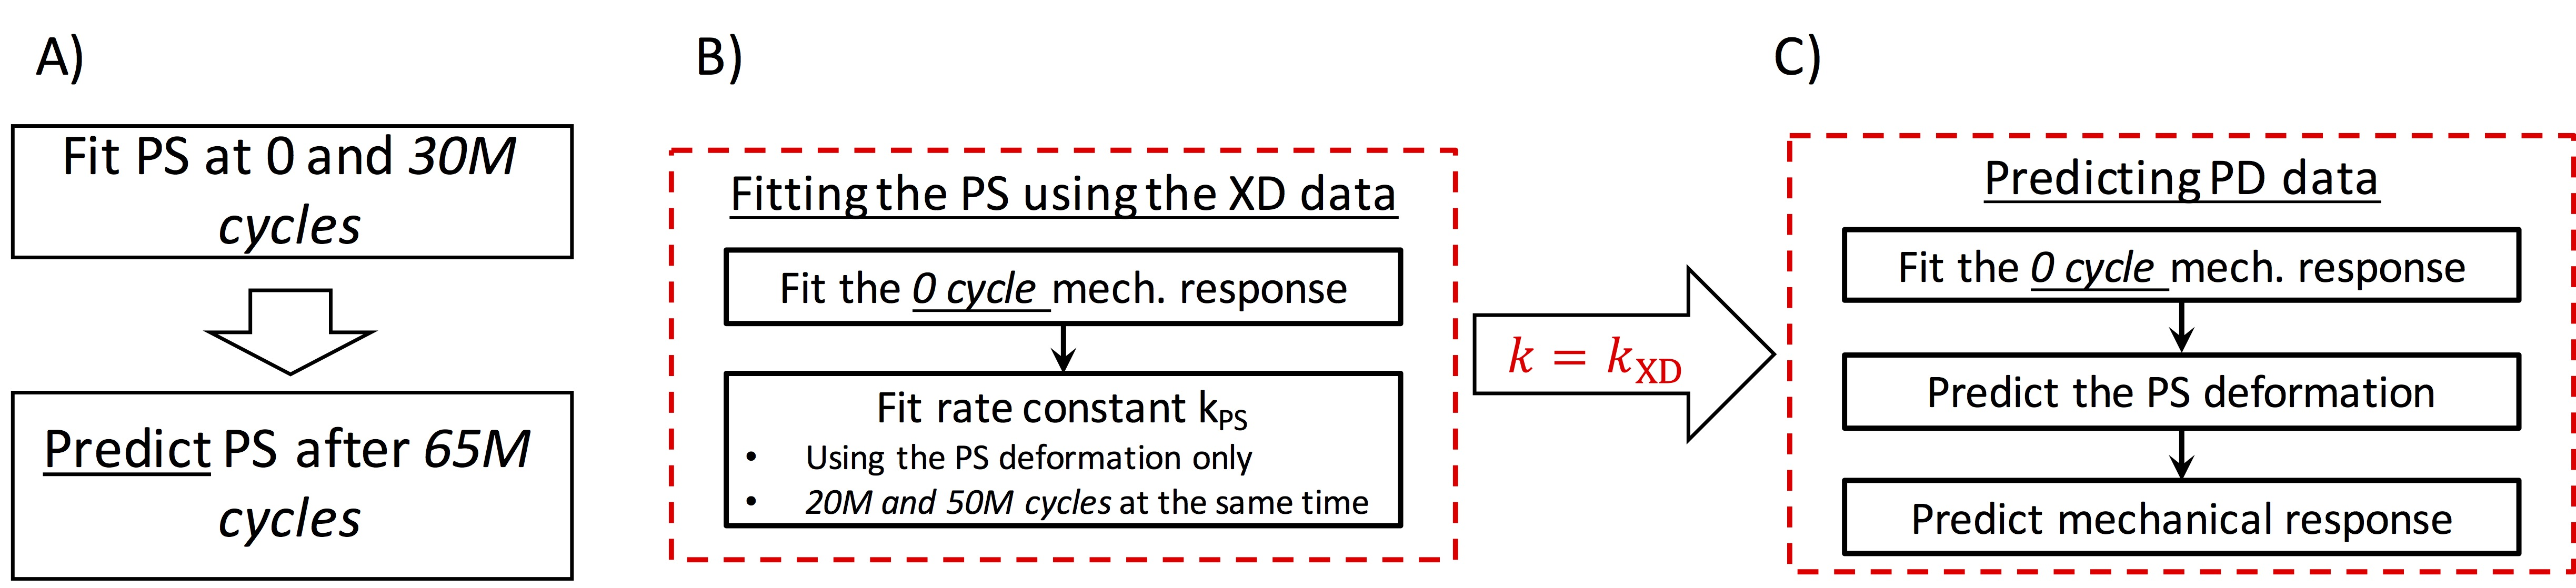
\includegraphics[width=\textwidth]{Images/chapter4/figure12}}
\caption{Our parameter estimation approach for the A) strain controlled cyclic loading data, B) stress controlled data cycled in the cross-preferred direction and C) in the preferred direction}
\label{fig:datamethods}
\end{figure}


%%%%%%%%%%%%%%%%%%%%%%%%%%%%%%%%%%%%%%%%%%%%%%%%%%%%%%%%%%%%
%%%%    Stress controlled cycling

\subsubsection{Stress controlled cycling}
The parameter estimation for the stress controlled specimens is more complicated than the strain controlled specimens as we do not know the strain history \textit{a priori}. This becomes a dynamic simulation, and we need to use optimization to determine the strain history (Eqn. \ref{eq:optimization}) at each time point. Thus, this data set is well suited to validate the full model using time dependent simulations. Since we have data for both PD-loading and XD-loading, we can fit the XD-loading data and used the resulting rate constant $k $ to predict the PD-loading data. First, we discretized the problem as followed
\begin{equation} 
\begin{aligned}
\phi_m \mathbf{S}_m =& \phi_m \left[\mathrm{Exp} \left[-k  \cdot n \cdot \Delta s \right] \mathbf{\bar{S}}_m \left(\mathbf{F}_\mathrm{PS}, \mathbf{I},\mathbf{C}\right)\vphantom{\sum_{i = 1}^n}\right. \\
&+ \left.\sum_{i = 1}^n  (k \Delta s) \mathrm{Exp}\left[-k (n\Delta s - i \Delta s)\right] \mathbf{\bar{S}}_m \left(\mathbf{F}_\mathrm{PS}, \mathbf{A}(i\Delta s),\mathbf{C}\right)\right].
\end{aligned}
\end{equation}
After each time step $\Delta s$, we compute the new loaded state $\mathbf{A}(i\Delta s)$ using optimization(Eqn. \ref{eq:optimization}, Fig. \ref{fig:implementation}). Through preliminary trials, the most optimal resolution in time is $\Delta s = 1$ million cycles when considering both time to run the simulations and accuracy of the results. We note that since an additional optimization is added to the parameter estimation process, we can no longer fit both the permanent set deformation $\mathbf{F}_\mathrm{PS}$ and the mechanical data at the same time. Our attempts at fitting both at the same time were not able to converge. Thus, we choose to predict the mechanical data as a way to validate our results. 
The parameter estimation process for the XD-loading data is
\begin{enumerate}
\item Determine the 0-cycled mechanical response
\item Fit the permanent set deformation $\mathbf{F}_\mathrm{PS}$ 
	\begin{enumerate}
	\item choose a $k $
	\item choose a mounting direction $\theta_\mathrm{mount}^{20}$ for cycling up to 20 million cycles 
	\item compute $err_\mathrm{PS} = \mathbf{F}_\mathrm{PS} - \mathbf{F}_\mathrm{PS}^\mathrm{data}$ error at 20 million cycles
	\item choose a mounting direction $\theta_\mathrm{mount}^{50}$ for cycling from 20 to 50 million cycles 
	\item compute $err_\mathrm{PS} = \mathbf{F}_\mathrm{PS} - \mathbf{F}_\mathrm{PS}^\mathrm{data}$ error at 50 million cycles
	\item update $k$, $\theta_\mathrm{mount}^{20}$, and $\theta_\mathrm{mount}^{50}$ using Quasi-Newton
	\end{enumerate}
\item Predict the mechanical response 
\end{enumerate}
Next we, used $k $ from the XD-loading data to predict the PD-loading data. 
\begin{enumerate}
\item Determine the 0-cycled mechanical response
\item Compute Fit the permanent set deformation $\mathbf{F}_\mathrm{PS}$
	\begin{enumerate}
	\item set $k $ from XD-loading data
	\item choose a mounting direction $\theta_\mathrm{mount}^{20}$ for cycling up to 20 million cycles 
	\item compute $err_\mathrm{PS} = \mathbf{F}_\mathrm{PS} - \mathbf{F}_\mathrm{PS}^\mathrm{data}$ error at 20 million cycles
	\item choose a mounting direction $\theta_\mathrm{mount}^{50}$ for cycling from 20 to 50 million cycles 
	\item compute $err_\mathrm{PS} = \mathbf{F}_\mathrm{PS} - \mathbf{F}_\mathrm{PS}^\mathrm{data}$ error at 50 million cycles
	\item update $\theta_\mathrm{mount}^{20}$ and $\theta_\mathrm{mount}^{50}$ using Quasi-Newton
	\end{enumerate}
\item Predict the mechanical response 
\end{enumerate}

%%%%%%%%%%%%%%%%%%%%%%%%%%%%%%%%%%%%%%%%%%%%%%%%%%%%%%%%%%%%%%%%%%%%%%%%%%%%%%%%
%%%%    Parametric studies


\begin{figure}[hbt]
\centering
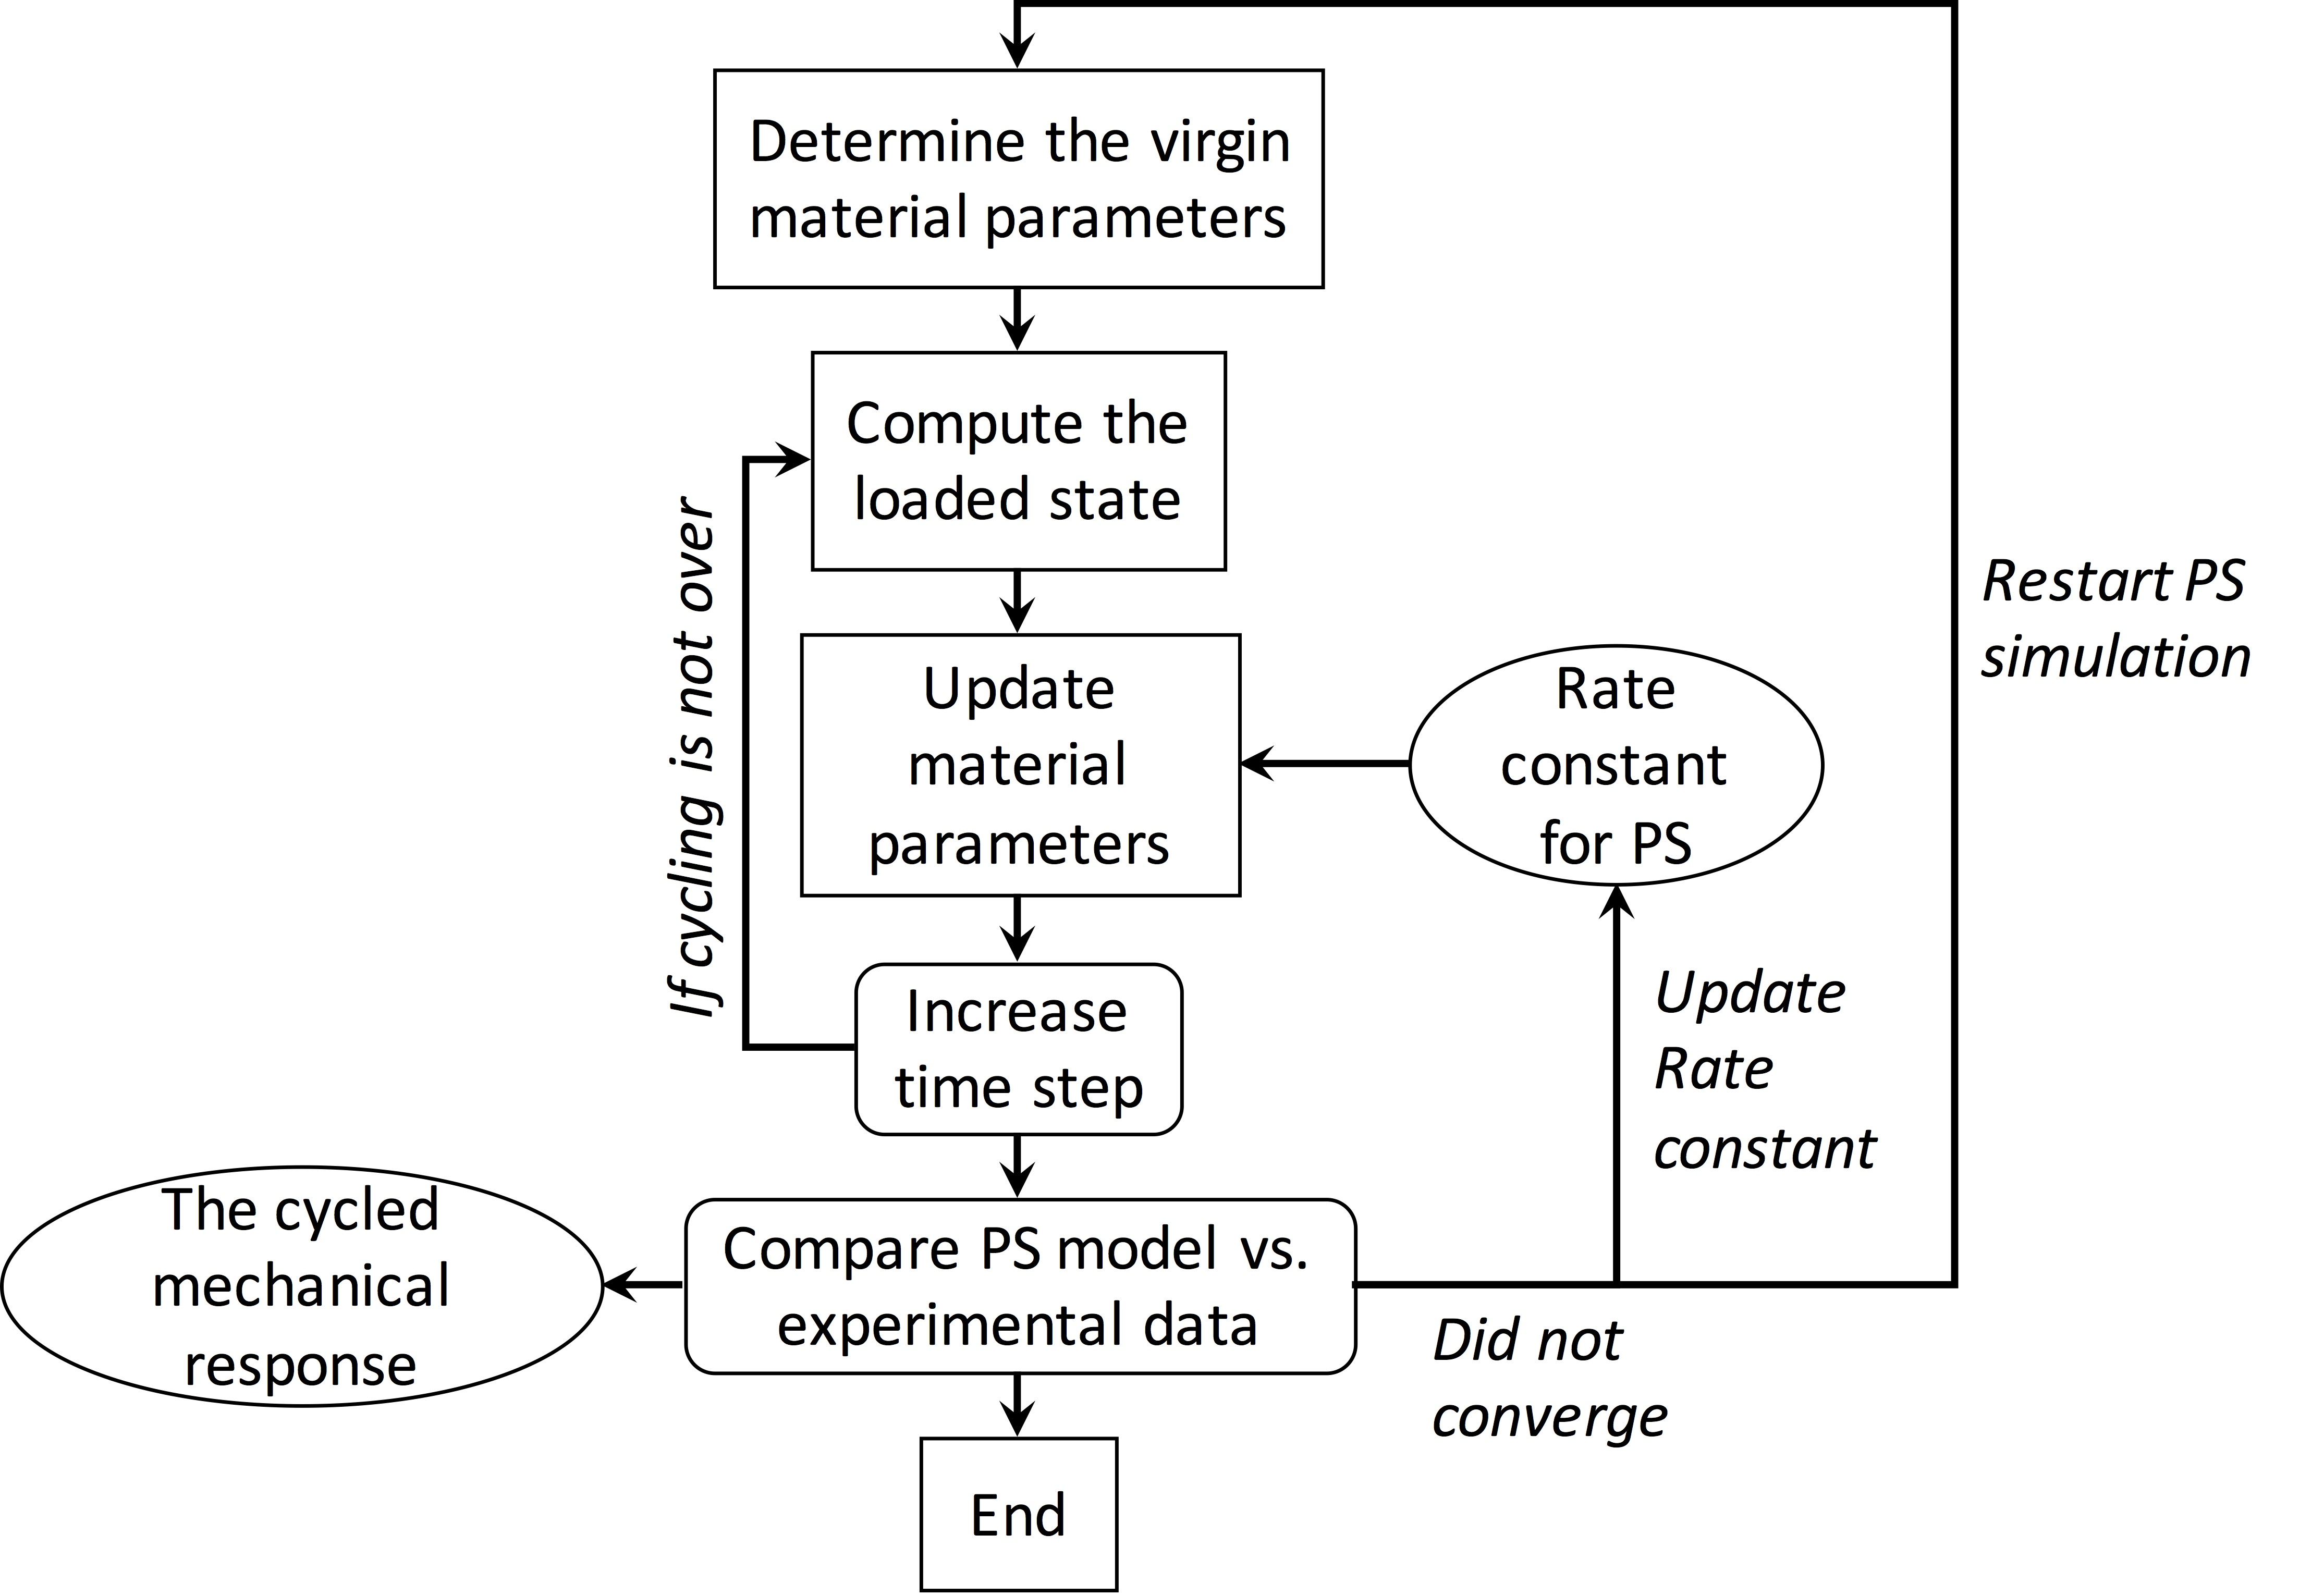
\includegraphics[width=5in]{Images/chapter4/figure13}
\caption{Implementation of the full model with updates in time.}
\label{fig:implementation}
\end{figure}


\subsection{Parametric studies}
Next, we performed an parametric study using the stress-controlled PD data. The same material parameters and rate constant, $k$, from parameter estimation results above was used. We simulated one specimen by extending the cycle duration to 100 million cycles to examine how the changes in geometry due to permanent set respond to an extended cycling period. 